\chapter{Ultracold atomic gases}
\label{cha:cold-gases}

\section{Bose-Einstein condensation}
\label{sec:BEC}


\paragraph{BEC in noninteracting gas}
In 1925, Albert Einstein (prompted by the earlier work of the indian
polyglot Satyendra Nath Bose) considered what would happen to a
non-interacting bosonic gas of non-relativistic particles in the
thermodynamic limit, as one lowers the temperature. He predicted the
phenomenon we now call \textit{Bose-Einstein condensation} (BEC),
namely a phase transition to a new state of matter, in which a finite
fraction of all the particles would occupy the same single-particle
state. The transition occurs at fixed density below a critical
temperature $T_c$ or, alternatively, at fixed temperature, above a
critical density. In particular, if we take $N$ neutral particles in a
cubic box of volume $L^3$, then they would predominantly occupy the
zero-wavevector state $\kv = 0$, and the critical temperature would
be~\cite{9780198507192}
%
\begin{equation}\label{eq:Tc3D}
  T_c \simeq 3.31 \frac{\rho^{2/3}\hbar^2}{m k_B}
\end{equation}
%
with the density $\rho = N/L^3$ and $m$, $k_B$ being the particle
mass and Boltzmann's constant, respectively.

At its core, BEC is a paradigm of quantum statistical mechanics,
stemming from the indistinguishability of elementary particles and the
Bose-Einstein statistics that they obey. One can hand-wavingly deduce
the critical temperature (or critical density) where quantum
degeneracy would start playing a role in a many-body system, by
arguing that the thermal de Broglie wavelength should be comparable to
or greater than the inter-particle distance (which in our case is
$\rho^{-1/3}$ on average)~\cite{Leggett_1999}. Apart from the
numerical prefactor, we get the same answer as
Eq.~\eqref{eq:Tc3D}. While one may argue that elementary massive
bosons do not exist, it is worth emphasizing that indistinguishability
only plays a role when there is a finite probability for exchange
processes to occur between the particles. In that sense, all
odd-isotope alkali atoms under relevant experimental conditions (see
below) effectively behave as bosons: their many-body wavefunction is
symmetric under the exchange of any two such atoms.

\paragraph{BEC in interacting system}
Interestingly enough, BEC was considered by many at the time to be a
pathological behaviour of the non-interacting gas, which would resolve
once interactions were properly accounted for. In fact, it is well
known that the ideal Bose gas has infinite compresibility.  This
pathology is cured by introducing a weak repulsive interaction between
bosons, a regime where BEC survives, as we will see next.

\paragraph{One-body density matrix}
Following Leggett, we characterise each of the $N$ particles (assumed
spinless, for simplicity) by a position vector $\rv_i$, with the label
$i$ running from 1 to $N$. Any pure state $s$ of the (now interacting)
system -- which can be also subjected to an external potential -- can
be described at time $t$ by the many-body wavefunction
$\Psi_s(\rv_1,\rv_2,\dots,\rv_N,t)$. Therefore, the most general state
of the system (also called \textit{mixed state}) can be written as a
superposition of pure orthonormal states $s$ with different weights
$p_s$. The \textit{single-particle density matrix}
$\hat{\rho}_1(\rv,\rv^{\prime},t)$ represents the probability
amplitude, at time $t$, of finding a specific particle at position
$\rv$, multiplied by the amplitude of finding it at $\rv^{\prime}$,
and averaged over the positions of all the other particles:
%
\begin{align}\label{eq:one-particle-rho}
  \hat{\rho}_1(\rv,\rv^{\prime},t) & \equiv N \sum_s p_s \int d\rv_2d\rv_3\dots
d\rv_N
\Psi_s^{\star}(\rv,\rv_2,\dots,\rv_N,t)\Psi_s(\rv^{\prime},\rv_2,\dots,\rv_N,t)\nonumber\\
& = \sum_i n_i(t) \phi_i^{\star}(\rv,t) \phi_i(\rv^{\prime},t)
\end{align}
% 
where in the second line we have re-written the density matrix in
diagonal form, introducing its eigenvalues $n_i$ and eigenvectors
$\phi_i$, which form a complete orthonormal set at any time $t$ (here
$i$ labels a good quantum number of the problem, i.e. momentum in a
translationally-symmetric situation).

\paragraph{Penrose-Onsager criterion for BEC}
We are now ready to state the Penrose-Onsager criterion for
condensation, first formulated in 1956: if at any given time $t$ it is
possible to find a complete orthonormal basis of states of
$\hat{\rho}_1$ such that one and only one of these states has an
eigenvalue of order $N$ (the rest being of order 1), then we say the
system exhibits BEC. One should note that this definition only applies
to ``simple'' BEC, as opposed to the ``fragmented'' case (of no
concern to us here), where two or more of the eigenvalues of the
one-body density matrix are of order $N$.

\paragraph{Condensate wavefunction and the order parameter}
We denote the single macroscopic eigenvalue of the density matrix by
$N_0(t)$, and its corresponding eigenfunction by
$\phi_0(\rv,t)$. $\phi_0$ is called the \textit{condensate
  wavefunction} and the $N_0$ particles occupying it the
\textit{condensate}, while the ratio $N_0/N$ is the \textit{condensate
  fraction}. It is not necessarily true that $N_0 = N$, even at zero
temperature. Also note that, while $\phi_0$ behaves as a
single-particle Schr\"{o}dinger wavefunction, it is generally not an
eigenfunction of the single-particle part of the Hamiltonian, or of
any other simple operator for that matter, other than
$\hat{\rho}_1$. Another useful quantity frequently found in the
literature is the so-called \textit{order parameter},
$\psi(\rv,t) = \sqrt{N_0(t)}\phi_0(\rv,t)$. We see that, while
$\phi_0$ is normalized to 1, $\psi$ will be normalized to $N_0(t)$.

\paragraph{No-go theorem for lower dimensionality}
It is worth mentioning the existence of a theorem due to
Hohenberg~\cite{PhysRev.158.383}, stating that, in the thermodynamic
limit, BEC cannot occur at a finite temperature in any system moving
freely in space in less than three dimensions, irespective of the
existence and/or sign of the interparticle interactions, as thermal
fluctuations would destroy the condensate. Note that this theorem,
however, only applies under equilibrium conditions, the nonequilibrium
case still being an open question.  Furthermore, there is no general
proof that a realistic system of interacting bosonic particles must
show BEC, even at zero temperature -- the solid phase of ${}^4$He
constitutes an obvious counter-example.

\paragraph{Experimental proof}
Most gases, with the notable exception of ${}^4$He, are solids at the
densities and temperatures predicted by Eq.~\eqref{eq:Tc3D}. That is
why it took no less than 70 years between Einstein's original paper
and the first experimental observation of BEC in an atomic gas. In
1995, the group of Eric Cornell and Carl Wieman succesfully condensed
a cloud of ${}^{87}$Rb atoms~\cite{Anderson198} (closely followed by
the group of Wolfgang Ketterle at MIT with ${}^{23}$Na
atoms~\cite{PhysRevLett.75.3969}), by first bringing the system to a
very low density, and then cooling it fast enough to prevent any
recombination processes that would have lead to the formation of the
solid phase. While other odd-isotope alkali elements, especially
${}^{23}$Na or ${}^{7}$Li, are also routinely used in experiments, the
first non-alkali atom to be cooled into the BEC phase was hydrogen
${}^1$H. Due to the extreme diluteness of these systems
($\rho < 10^{15}$ atoms/cm${}^3$), the typical range of $T_c$ is from
$20$ nK to a few $\mu$K. Achieving such ultra-low temperatures
stimulated the development of novel experimental techniques, such as
magnetic/laser trapping and evaporative cooling of atoms.

\paragraph{Diagnostic techniques}
The very low densities of alkali gases also limit the range of
available diagnostic techniques. The most commonly employed method in
BEC experiments is optical absorption imaging, where one shines a
laser on the gas and detects the percentage of transmitted power. The
image is usually taken after removing the trap and allowing the gas to
expand. This gives information about the gas density as a function of
coordinates and time, with a spatial resolution of a few $\mu$m. In
stark contrast to liquid ${}^4$He, density-related information seems
to be sufficient for most practical purposes.

\paragraph{Diluteness/weak interaction condition}


\section{Gross-Pitaevskii equation}
\label{sec:GPE}

\paragraph{Short history and utility of GP equation}
As it turns out, many of the experimental results in ultracold gases
can be interpreted on the basis of a single equation for the
condensate wavefunction $\phi_0(\rv,t)$. This equation, first derived
in 1961 independently by Eugene Gross and Lev Pitaevskii, was
originally intended as a phenomenological description of quantum
vortices in the superfluid phase of liquid ${}^4$He, below the lambda
point. Since liquid helium is a strongly interacting system however,
the GP equation turned out to be much better suited to alkali gases.
Before giving the concrete formulation of the GP equation, we must
first explore the nature of the inter-atomic interactions.

\paragraph{s-wave scattering length}
In dilute systems, the inter-atomic distance $d = \rho^{-1/3}$ is on
the order of 1000~\AA, while the range $r_0$ of the inter-atomic
potential, namely the extent of the last bound state of the van der
Waals interaction, is about 50-100~\AA. As $d \gg r_0$, the
probability of three-atom colissions is substantially diminished. This
justifies limiting ourselves to a binary (instead of three-body or
more) scattering problem: consider two atoms, separated by a relative
distance $r$ and interacting in three dimensions through a potential
$V(r)$. We can therefore decouple their center-of-mass motion from
their relative one and write a Schr\"{o}dinger equation for the
scattering states $\psi(r)$.

For temperatures below $T_c$, the thermal de Broglie wavelength
$\lambda_T > d$ (as mentioned in Sec.~\ref{sec:BEC}), meaning all
significantly occupied states will have small wavevectors,
$k \ll r_0^{-1}$. This directly translates to a low relative kinetic
energy, and hence small relative wavevectors, for the scattering
problem outlined above. However, we know from scattering theory that
the probability for two atoms, with relative angular momentum $\ell$,
of being separated by a distance $r \ll k^{-1}$ is proportional to
$(kr)^{2\ell}$, therefore essentially negligible in the limit
$k r_0 \ll 1$. That is of course, unless $\ell = 0$, meaning their
relative state is $s$-wave, which is what we will assume from now
on. Since $r_0 \ll d$, one can use the asymptotic expression for
$\psi(r)$, which only depends on the scattering amplitude. At small
wavevectors, this amplitude can be safely replaced by the
\textit{$s$-wave scattering length} $a_s$, which will encapsulate all
the interaction effects on macroscopic properties of the atomic gas.

One can now replace the two-body potential $V(r)$ with an effective
interaction, $V_{\text{eff}}(r)$, provided it gives the same
scattering length. The limit of small wavevectors prompts us to only
consider the lowest Fourier component of $V_{\text{eff}}$, equivalent
in real space to a contact interaction\footnote{Technically, one
  should also include a regularizing part in order to remove any $1/r$
  divergencies of the wavefunction.}
$V_{\text{eff}}(r) = g \delta(r)$, where we have introduced the
interaction coupling constant $g$, whose value can be calculated using
the first-order Born approximation~\cite{9780198507192} 
%
\begin{equation}\label{eq:g-constant}
  g = \frac{4\pi\hbar^2}{m} a_s
\end{equation}
% 
The scattering length $a_s$ therefore becomes the small parameter of
the theory of weakly-interacting ultracold gases, and the validity of
the Born approximation rests on the following two conditions
%
\begin{align}
  k \abs{a_s} & \ll 1\\
    \abs{a_s} & \ll \rho^{-1/3}\label{eq:diluteness-condition}
\end{align}
% 
Eq.~\eqref{eq:diluteness-condition} is called the ``diluteness
condition'', and it paves the way to various mean-field approaches,
such as the GP equation.


\paragraph{Derivation of Gross Pitaevskii equation}
Formally, the GP equation corresponds to the lowest-order expansion in
$a_s$ of the more exact Bogoliubov theory. However, we will try to
give a hand-waving justification of it for the zero-temperature
case. At $T=0$, all $N$ particles are in the condensate, therefore one
could neglect all inter-particle correlations and introduce the
simplest (Hartree-Fock) ansatz, expressing the ground state many-body
wavefunction $\Psi$ in the symmetrized form
%
\begin{equation}\label{eq:HF-ansatz}
  \Psi(\rv_1,\rv_2,\dots,\rv_N,t) = \prod_{i = 1}^{N} \phi_0(\rv_i,t)
\end{equation}
% 
As mentioned in Sec.~\ref{sec:BEC}, the single-particle state $\phi_0$
(now occupied by all the bosons) obeys a Schr\"{o}dinger-like
equation, to which we must add the energy of the effective binary
interactions. In mean-field, these interactions contribute the
equivalent of a one-particle potential term proportional to
$\abs{\phi_0}^2$.~\cite{Leggett_1999} Together with the kinetic part,
this results in the nonlinear equation\footnote{We have tacitly
  assumed that $N$ is large enough, such that $N-1 \approx N$.}
%
\begin{equation}\label{eq:TDGP}
  i\hbar\partial_t\phi_0(\rv,t) = 
  \left[-\frac{\hbar^2\nabla^2}{2m} + U(\rv,t) + g N |\phi_0(\rv,t)|^2\right]\phi_0(\rv,t)
\end{equation}
% 
where we have also included an external potential $U(\rv,t)$, normally
used to model harmonic trapping of the gas. Note that
Eq.~\eqref{eq:TDGP} is valid for physics occuring over distances much
larger than the scattering length $a_s$, which in turn must be smaller
than the typical range $r_0$ of the potential $U(\rv,t)$.

\paragraph{Caveats of TDGP}
Eq.~\eqref{eq:TDGP} is the time-dependent Gross-Pitaevskii (TDGP)
equation, a mean-field result where the condensate wavefunction
$\phi_0$ must be calculated self-consistently. It is important to
emphasize that the TDGP equation is also valid at nonzero temperatures
$T \ll T_c$, provided that the density of non-condensed particles is
much smaller than the condensate density. In that case, the condensate
number $N_0$ is smaller (but still on the order of) the total particle
number $N$. Finally, one must note that the nonlinearity of
Eq.~\eqref{eq:TDGP} builds a bridge connecting BEC to nonlinear
optics, where a similar relation is used, under the name of
\textit{nonlinear Schr\"{o}dinger equation}.

\paragraph{Time-independent GP}
In case the external potential $U$ does not depend explicitly on time,
the stationary solutions of Eq.~\eqref{eq:TDGP} evolve with a trivial
phase factor $\exp(-i\mu t/\hbar)$. This yields a time-independent GP
equation for $\phi_0(\rv)$ (we set $\hbar = 1$ from here on)
%
\begin{equation}\label{eq:TIGP}
  \mu\phi_0(\rv) = \left[-\frac{\nabla^2}{2m} + U(\rv)+
    g N_0 |\phi_0(\rv)|^2\right]\phi_0(\rv)
\end{equation}
where $\mu$ is chemical potential of the gas, the energy required to
add one more particle to the system.\footnote{Technically, it is the
  Lagrange multiplier associated to the conservation of particle
  number $N_0$, and can be shown to be very close to the actual
  chemical potential in the thermodynamic limit.~\cite{9783540410478}}


\section{Linear response theory}
\label{sec:linear-response}

Following loosely the formalism presented in Ref.~\cite{9783540410478}, we now let $\phi_0(\rv)$ be the steady state solution to the GP equation in
the time-independent trapping potential $U_0(\rv)$
%
\begin{equation}\label{eq:GP-atoms}
  H_{\text{GP}} \phi_0 = 0
\end{equation}
% 
with the GP Hamiltonian defined as
%
\begin{equation}\label{eq:GP-ham}
  H_{\text{GP}} \equiv -\frac{\nabla^2}{2m} + U_0 + gN_0\abs{\phi_0}^2 - \mu
\end{equation}
% 
This Hamiltonian describes a bosonic condensate of $N_0$ particles
with contact interactions quantified by $g$, and chemical potential
$\mu$.  Now consider adding a small time-dependent perturbation on top
of the trap, giving $U(\rv,t)=U_0(\rv) + \delta U(\rv,t)$. We are
interested in the response of the condensate to this perturbation.
For weak perturbations, we can perform a linearization of the GP
equation Eq.~\eqref{eq:GP-atoms} around the stationary solution
$\phi_0$ -- an approach known in the literature as the ``linear
response'' formalism. The condensate wavefunction $\phi(\rv,t)$
evolves according to
%
\begin{equation}\label{eq:GP-atoms-evolution}
  i\partial_t \phi = \left[-\frac{\nabla^2}{2m} + U + gN_0 \abs{\phi}^2 - \mu\right] \phi
\end{equation}
% 
We assume a small deviation of the wavefunction from its initial
steady state
%
\begin{equation}\label{eq:ansatz-atoms}
  \phi(\rv,t) = \phi_0(\rv) + \delta\phi(\rv,t)
\end{equation}
% 
such that we can expand Eq.~\eqref{eq:GP-atoms-evolution} and keep only linear terms in $\delta\phi$ and $\delta U$. We get
%
\begin{equation}\label{eq:GP-atoms-lin}
  i\partial_t\delta\phi =  \left[-\frac{\nabla^2}{2m} + U_0-\mu\right]
  \delta\phi + 2 g N_0 \phi_0^{\star}\phi_0\delta\phi + gN_0\phi_0^2\delta\phi^{\star}
  +\delta U\phi_0
\end{equation}
% 
Note that Eq.~\eqref{eq:GP-atoms-lin} is not strictly linear due to
the coupling of $\delta\phi$ to $\delta\phi^{\star}$. To restore
linearity, we consider the functions $\delta\phi$ and
$\delta\phi^{\star}$ as being independent and write the linear system
%
\begin{equation}\label{eq:GP-atoms-system}
  i \partial_t \colvec{\delta\phi(\rv,t)}{\delta\phi^{\star}(\rv,t)}
  = \Lca_{GP} \colvec{\delta\phi(\rv,t)}{\delta\phi^{\star}(\rv,t)}
  + \colvec{S(\rv,t)}{-S^{\star}(\rv,t)}
\end{equation}
% 
where we have introduced the linear operator
%
\begin{equation}\label{eq:LGP}
  \Lca_{\text{GP}} = \mat{H_{\text{GP}}+gN_0\abs{\phi_0}^2}{g N_0 \phi_0^2}{-g N_0 \phi_0^{\star 2}}{-\left[H_{\text{GP}}+gN_0\abs{\phi_0}^2\right]^{\star}}
\end{equation}
% 
and the source term $S(\rv,t)=\delta U(\rv,t)\phi_0(\rv)$.  Note that
$\Lca_{\text{GP}}$ is a non-Hermitian operator!

We now consider the eigenvalue equation for the operator $\Lca_{\text{GP}}$
%
\begin{equation}\label{eq:L-eigen}
  \Lca_{\text{GP}} \ket{\psi_k^R} = \epsilon_k \ket{\psi_k^R}
\end{equation}
% 
with $\ket{\psi_k^R}$ being the right eigenvector and $\epsilon_k$ its
corresponding eigenvalue
%
\begin{equation}\label{eq:psi-R}
  \ket{\psi_k^R} = \colvec{\ket{u_k}}{\ket{v_k}}
\end{equation}
% 
Similarly, we also introduce the left eigenvector, obeying
$\Lca_{\text{GP}}^{\dagger} \ket{\psi_k^L} = \epsilon_k^{\star} \ket{\psi_k^L}$,
and the orthonormality condition
$\braket{\psi_k^L}{\psi_q^R} = \delta_{k,q}$. 

Notice that $\Lca_{\text{GP}}$ and $\Lca_{\text{GP}}^{\dagger}$ are
connected by the unitary transformation\footnote{Note that this holds
  as long as the Hamiltonian $H_{\text{GP}}$ only contains real
  terms.}
%
\begin{equation}\label{eq:symmetry-1}
  \eta \Lca_{\text{GP}} \eta^{\dagger} = \Lca_{\text{GP}}^{\dagger}
\end{equation}
% 
where $\eta = \sigma_3 = \mat{1}{0}{0}{-1}$ is the third Pauli
matrix. We say that $\Lca_{\text{GP}}$ is $\eta$-Hermitian, meaning
that one can define a new scalar product
$\braket{\cdot}{\cdot}_{\eta} \equiv \braket{\cdot}{\eta \cdot}$ with a
different signature, such that
$\braket{\cdot}{\Lca_{\text{GP}} \cdot}_{\eta} =
\braket{\Lca_{\text{GP}} \cdot}{\cdot}_{\eta}$. The operator $\eta$ is
usually called the metric operator, and, not suprisingly in our case,
it is the same as the one of the scalar Klein-Gordon equation. A
pseudo-Hermitian operator usually also posesses antilinear symmetries,
and as we will see below this is also the case for
$\Lca_{\text{GP}}$. Interestingly, for operators with a real spectrum,
it can be shown that one can define another metric $\eta_+$, which
guarantees a positive-definite inner product, or, in other words,
$\braket{\psi}{\psi}_{\eta_+} > 0$ (provided $\psi \neq 0$ of
course). This can be used to formulate a probabilistic quantum theory
for the new wave-functions $\psi^R$ and $\psi^L$. For the general
theory and properties of pseudo-Hermitian operators, we point the
interested reader to Ref.~\cite{MOSTAFAZADEH_2010}.


Using Eq.~\eqref{eq:symmetry-1}, we get the general form of the left
eigen-vectors as
%
\begin{equation}\label{eq:psi-L}
  \bra{\psi_k^L} = \mathcal{N}_k \left( \bra{u_k},\, -\bra{v_k} \right)
\end{equation}
% 
with $\mathcal{N}_k$ a normalization factor.  We can chose
$\mathcal{N}_k = \pm 1$ and group the eigenvalues of $\Lca_{\text{GP}}$
into 3 families, according to the quantity
%
\begin{equation}\label{eq:norms}
  n_k = \braket{u_k}{u_k} - \braket{v_k}{v_k}
\end{equation}
% 
We therefore have: the ``$+$'' family, corresponding to $n_k=+1$, the
``$-$'' family, such that $n_k=-1$ and the ``$0$'' family, with
$n_k=0$.

% In the absence of the added weak perturbation, the time evolution of
% mode $k$ is given by $\exp(-i\epsilon_k t)$, from which we get the
% dynamical stability condition $\imag{(\epsilon_k)} \leq 0$ for all
% $k$. Dynamical stability is important because it insures that small
% perturbations will not induce the condensate wavefunction to evolve
% far from its steady state value.

We are now ready to write the completeness relation
%
\begin{equation}\label{eq:completeness}
  \sum_k \ket{\psi_k^R} \bra{\psi_k^L} = \mathbb{I}
\end{equation}
% 
Using Eq.~\eqref{eq:completeness}, we can decompose any column vector
as\footnote{The modes in the ``$0$'' family do not appear in this
  expansion as their components live in the space orthogonal to the one
  of our solution.}
%
\begin{multline}\label{eq:decomposition}
  \colvec{\ket{l_1}}{\ket{l_2}} = \sum_{k \in ``+" \mbox{\scriptsize family}} \left[\braket{u_k}{l_1} - \braket{v_k}{l_2}\right]\colvec{\ket{u_k}}{\ket{v_k}}\\
  + \sum_{k \in ``-" \mbox{\scriptsize family}} \left[\braket{v_k}{l_2} - \braket{u_k}{l_1}\right]\colvec{\ket{u_k}}{\ket{v_k}}
\end{multline}
% 
There is now a further symmetry of $\Lca_{\text{GP}}$ that we can
exploit in our problem, a sort of time-reversal ``spin''-flip
symmetry, namely
%
\begin{equation}\label{eq:symmetry-2}
   \Theta \Lca_{\text{GP}} \Theta^{\dagger} = -\Lca_{\text{GP}}
\end{equation}
%
where $\Theta = \sigma_1 \mathcal{K}$, with
$\sigma_1 = \mat{0}{1}{1}{0}$ the first Pauli matrix and $\mathcal{K}$
the complex conjugation antilinear operator. This results in a
duality between the ``$+$'' family with eigenvectors $(u_k, v_k)$ and
energy $\epsilon_k$ and the ``$-$'' family with eigenvectors
$(v_{-k}^{\star}, u_{-k}^{\star})$ and energy
$-\epsilon_{-k}^{\star}$.

We can now finally project Eq.~\eqref{eq:GP-atoms-system} onto the
eigenvectors of $\Lca_{\text{GP}}$. Using the above-mentioned duality and
Eq.~\eqref{eq:decomposition}, we get
%
\begin{equation}\label{eq:phi-column-expansion}
  \colvec{\delta\phi(\rv,t)}{\delta\phi^{\star}(\rv,t)} = \sum_{k \in ``+" \mbox{\scriptsize family}}
  b_k(t) \colvec{u_k(\rv)}{v_k(\rv)}
  + b_{-k}^{\star}(t) \colvec{v_{-k}^{\star}(\rv)}{u_{-k}^{\star}(\rv)}
\end{equation}
% 
with the complex amplitudes $b_k$ satisfying 
%
\begin{equation}\label{eq:amplitudes-bk}
  i \frac{d}{dt}b_k(t) = \epsilon_k b_k(t) + s_k(t)
\end{equation}
% 
where we introduced
%
\begin{equation}\label{eq:amplitudes-sk}
  s_k(t) = \left( \bra{u_k} ,\, -\bra{v_k} \right) \colvec{\ket{S(t)}}{-\ket{S^{\star}(t)}}
\end{equation}
% 

\section{Cherenkov emission of Bogoliubov excitations}
\label{sec:cherenkov-emission}


We now turn to applying the formalism developed in
Sec.~\ref{sec:linear-response} to a concrete physical example, namely
a flowing condensate scattering against a static
defect~\cite{Carusotto_2006}. The BEC\footnote{We integrate all
  density profiles along the $z$ direction, resulting in an effective
  2-dimensional description.} is therefore in a state with
well-defined momentum, described by the plane wave
%
\begin{equation}\label{eq:atom-initial}
  \phi_0(\rv, t) = \psi_0 \exp \left( i \bm{k}_0 \rv - \omega_0 t \right)
\end{equation}
% 
and a chemical potential $\mu = k_0^2/(2m) + g \rho_0$. Since we have
no trap, $U_0(\rv)=0$, and Eq.~\eqref{eq:GP-atoms} produces the
equation of state
%
\begin{equation}\label{eq:atom-MF}
  \omega_0 - \left( \frac{k_0^2}{2m} + g \rho_0 \right) = 0
\end{equation}
% 
where we have introduced the condensate density
$\rho_0 \equiv N_0 \abs{\phi_0}^2$. 

We now introduce a weak perturbation in the form of a static localized
defect potential $\delta U(\rv, t) = V_d(\rv)$, which can represent
for instance a laser spot depleting a small area of the condensate, as
shown in Fig.~\ref{fig:mach-number}.
%
\begin{figure}[tb]\centering
  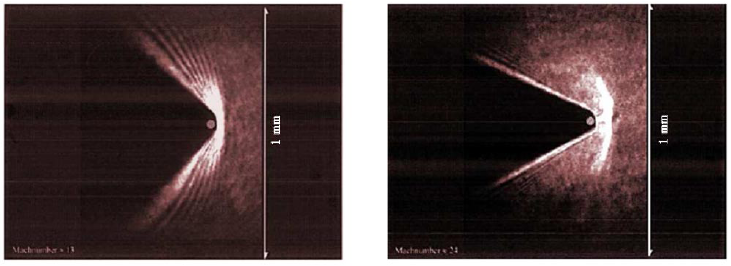
\includegraphics[width=.9\linewidth]{mach_number}
  \caption{
    % 
    Density profiles of an expanding BEC hitting a stationary defect
created by the repulsive potential of a blue-detuned laser beam. The
condensate has different speeds in the two panels, moving roughly
twice as fast in the right-panel. Notice the Mach cone formed behind
the defect, which gets narrower as the condesate moves faster. From
Ref.~\cite{Carusotto_2006}.
    % 
}\label{fig:mach-number}
\end{figure}
% 
\begin{figure}[tb]\centering
  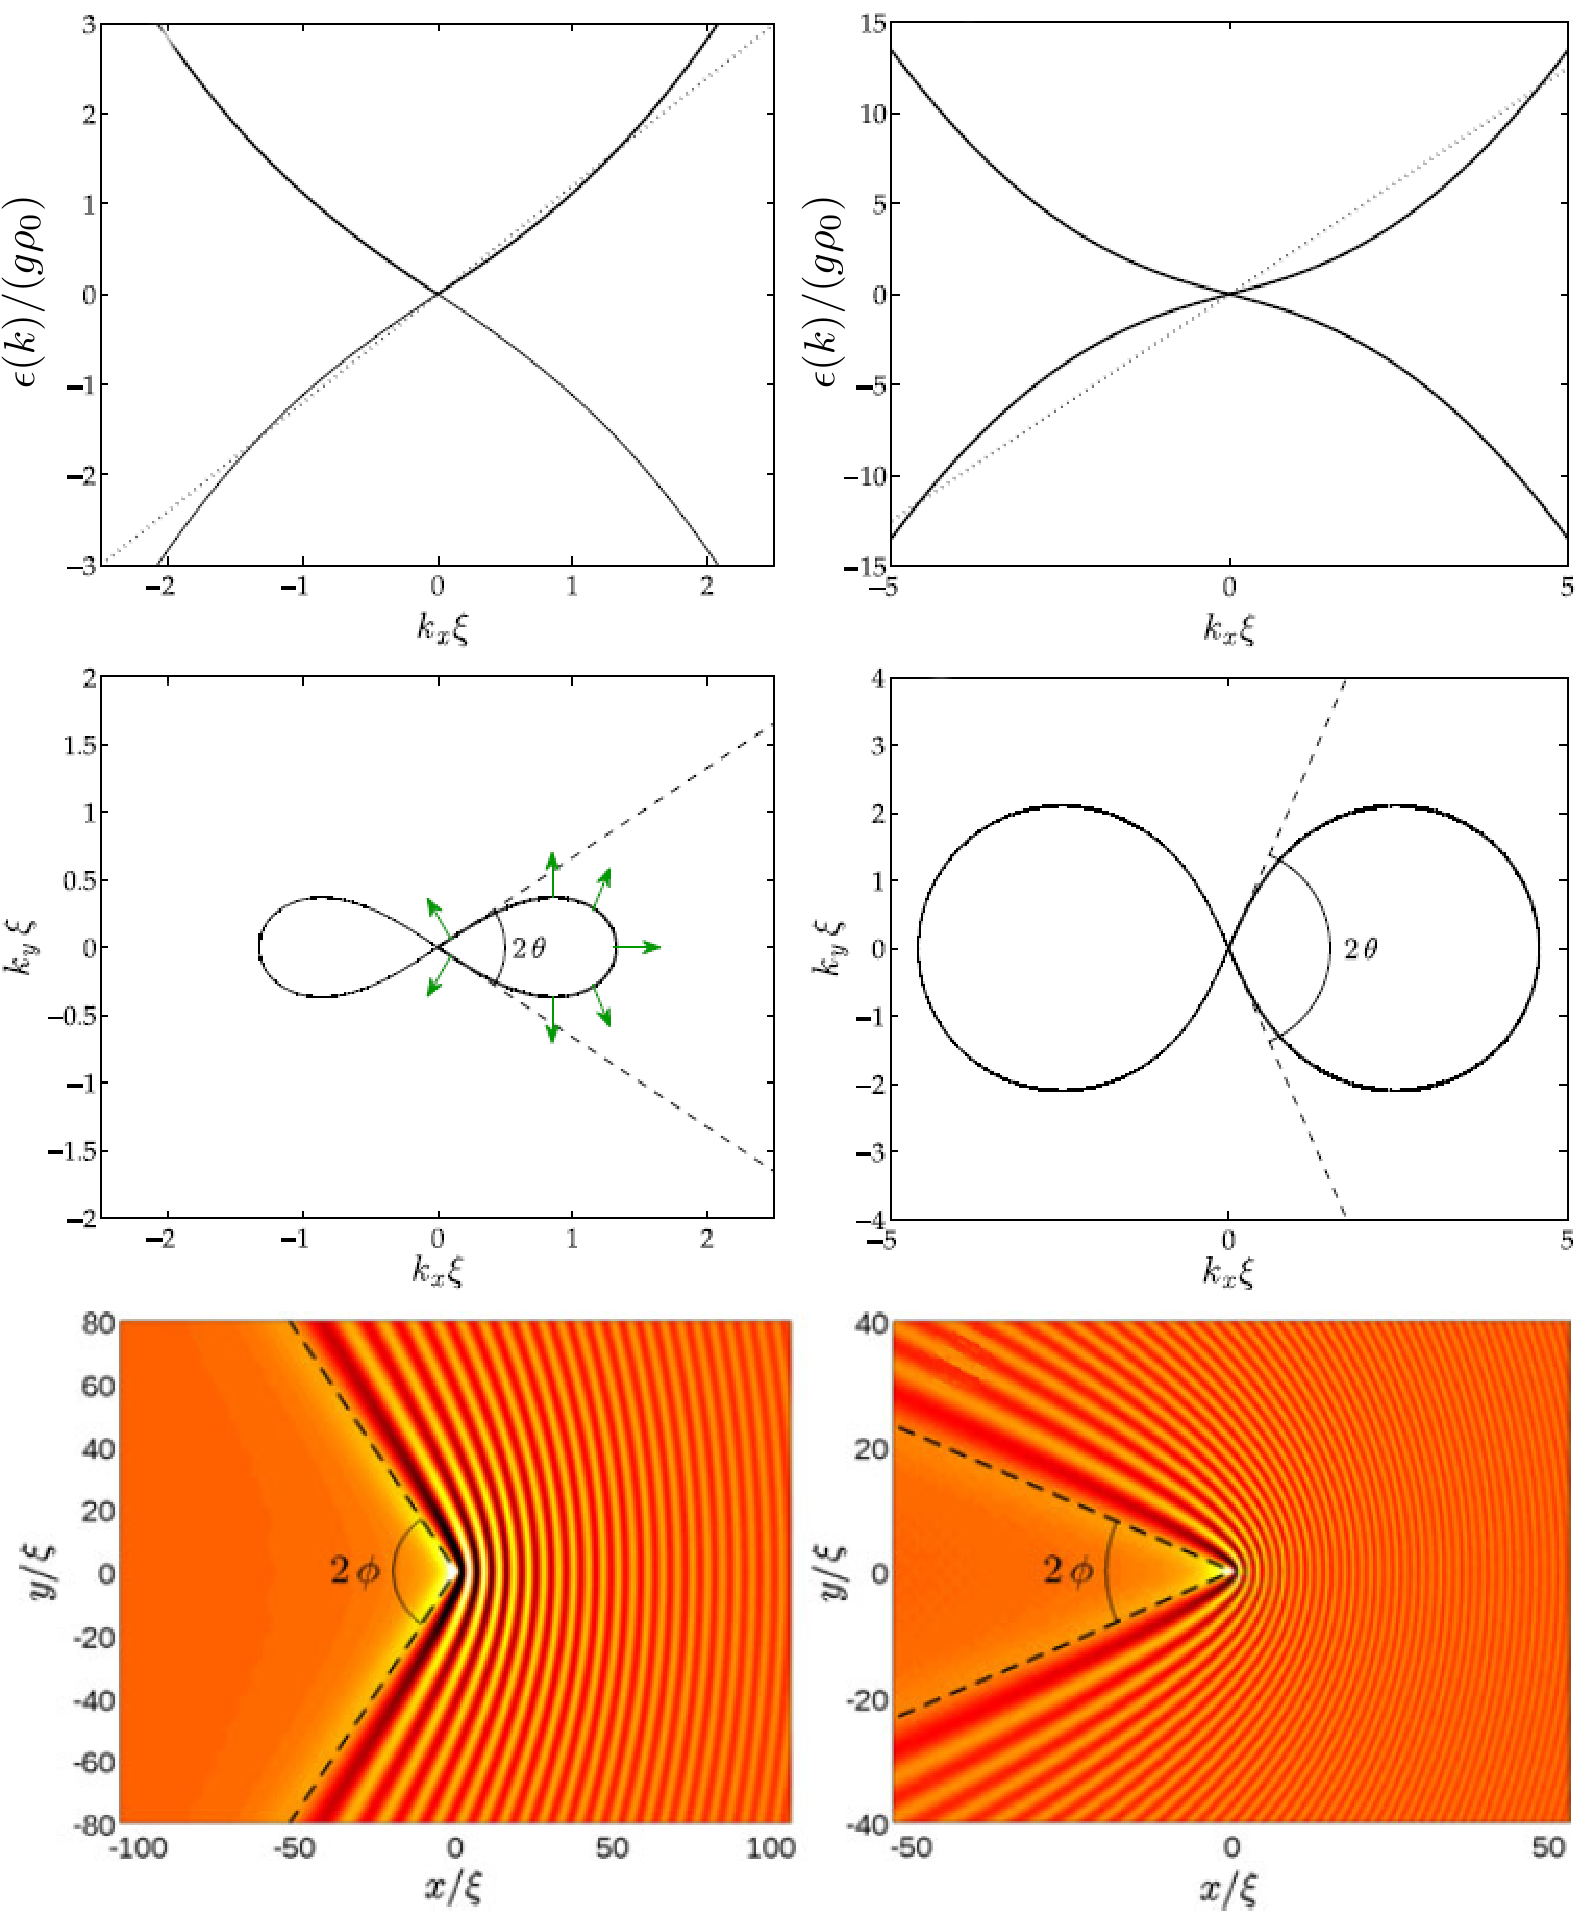
\includegraphics[width=.85\linewidth]{ducks_new}
  \caption{
    % 
    \emph{Top panels:} Bogoliubov dispersion
Eq.~\eqref{eq:bogoliubov}. The dotted lines indicate the $\bm{v}_0
\kv$ plane.
    \emph{Middle panels:} Locus $\Gamma$ of intersection of the 2D
dispersion with the $\bm{v}_0 \kv$ plane. Green arrows are normal
to $\Gamma$, while the dashed lines indicate the Cherenkov
cone.
    \emph{Bottom panels:} Real-space density modulation, with a
$\delta$--defect at $(0,0)$. Dashed lines show the Mach cone. Left
column panels are for $v_0 = 1.2 c_s$, and right column for $v_0 = 2.5
c_s$. From Ref.~\cite{9783319002651}.
    % 
}\label{fig:bogo-cherenkov}
\end{figure}

Using Eq.~\eqref{eq:atom-MF}, the GP Hamiltonian becomes
$H_{\text{GP}} = -\frac{\nabla^2}{2m} - \frac{k_0^2}{2m}$ and the
source term
$S(\rv) = \psi_0 V_d(\rv) \exp \left( i \bm{k_0} \rv \right)$. We now
get the linear operator for our problem in the form
%
\begin{equation}\label{eq:ourL}
  \Lca = \mat{-\frac{\nabla^2}{2m} - \frac{k_0^2}{2m} + g\rho_0}{g N_0 \psi_0^2 \exp \left( 2 i \bm{k_0} \rv \right)}{- g N_0 \psi_0^{\star 2} \exp \left( - 2 i \bm{k_0} \rv \right)}{-\left[ -\frac{\nabla^2}{2m} - \frac{k_0^2}{2m} + g\rho_0 \right]}
\end{equation}
% 
Notice that, due to the presence of the off-diagonal exponential
terms, $\Lca$ does not commute with the momentum operator, which is
the generator of the spatial translation group. Luckily, however, we
can restore translational invariance by a simple unitary
transformation, as shown below.

Using the standard commutation relations, one can show that, for a
constant wavevector $\bm{k_0}$, the unitary operator\footnote{The hat
  symbol denotes operators in the relevant Hilbert space.}
%
\begin{equation}\label{eq:trans-oper}
  \hat{T}(\bm{k_0}) = \exp \left( -i \bm{k_0} \hat{\rv} \right)
\end{equation}
% 
performs a translation in momentum space,
$\hat{T}(\bm{k_0}) \ket{\bm{k}} = \ket{\bm{k} - \bm{k_0}}$, with the
ket $\ket{\bm{k}}$ representing a single particle state with
wavevector $\bm{k}$ such that
$\hat{\bm{k}} \ket{\bm{k}} = \bm{k} \ket{\bm{k}}$. Using the
definitions above, one can easily obtain the commutator
%
\begin{equation}\label{eq:trans-commutator}
  \left[ \hat{\bm{k}},\, \hat{T}(\bm{k_0}) \right] = -\bm{k_0}\hat{T}(\bm{k_0}) 
\end{equation}
%
This allows us to rewrite the following expressions
\begin{align}\label{eq:products}
  \begin{split}
    \hat{T}^{\dagger}(\bm{k_0})\hat{\bm{k}}\hat{T}(\bm{k_0})& = \hat{\bm{k}} - \bm{k_0}\hat{\mathbb{I}}\\
    \hat{T}(\bm{k_0})\hat{\bm{k}}\hat{T}^{\dagger}(\bm{k_0})& = \hat{\bm{k}} + \bm{k_0}\hat{\mathbb{I}}  
  \end{split}
\end{align}

We now recognize the two exponentials in Eq.~\eqref{eq:ourL} as being
the real-space representation of $\hat{T}^2(\bm{k_0})$ and its
hermitian conjugate. This motivates us to define the following unitary
operator
%
\begin{equation}\label{eq:ucal}
  \hat{\mathcal{T}}(\bm{k_0}) = \mat{\hat{T}(\bm{k_0})}{0}{0}{\hat{T}^{\dagger}(\bm{k_0})}
\end{equation}
% 
such that a unitary transformation of our operator $\Lca$ now restores
translational symmetry. Indeed, one can see that
%
\begin{equation}\label{eq:translated-L}
  \hat{\mathcal{T}} \hat{\Lca} \hat{\mathcal{T}}^{\dagger} = \mat{\frac{\left(\kop + \bm{k_0}\right)^2}{2m} - \frac{k_0^2}{2m} + g\rho_0}{g N_0 \psi_0^2}{- g N_0 \psi_0^{\star 2}}{-\left[\frac{\left(\kop - \bm{k_0}\right)^2}{2m} - \frac{k_0^2}{2m} + g\rho_0 \right]}
\end{equation}
% 
where we have made use of Eqs.~\eqref{eq:products} and we have written
$\hat{\Lca}$ in a base-independent representation.  In the subspace of
momentum eigenstates $\ket{\kv}$, we can write the (right-)eigenvalue
equation corresponding to Eq.~\eqref{eq:translated-L} as
%
\begin{equation}\label{eq:right-eigen}
  \Lca_{\text{GP}} [k] \colvec{U_\sigma(k)}{V_\sigma(k)} = \epsilon_\sigma(k) \colvec{U_\sigma(k)}{V_\sigma(k)}
\end{equation}
% 
where we have recovered the matrix representation of
Eq.~\eqref{eq:LGP}, and introduced the notation
%
\begin{equation}\label{eq:boosted-bogoliubov}
  \omega_\sigma(\kv) = \bm{v}_0 \kv + \epsilon_\sigma(k)
\end{equation}
% 
Here $\sigma = \pm$ labels the 2 different eigenmodes, and we defined
the condensate speed $\bm{v}_0 \equiv \frac{\kv_0}{m}$.

Notice that the $k=0$ mode has only one eigenvector. However, one can
safely exclude it as this mode does not imply energy or momentum
transport. Excluding the $k = 0$ point, one can then solve
Eq.~\eqref{eq:right-eigen}, obtaining the celebrated Bogoliubov
excitation spectrum
%
\begin{equation}\label{eq:bogoliubov}
  \epsilon_\sigma(k) = \sigma \left[\frac{k^2}{2m}\left(\frac{k^2}{2m} + 2 g \rho_0 \right) \right]^{\frac{1}{2}}
\end{equation}
% 
with $\sigma = \pm$, as before. Here $k$ represents the momentum of
the quasiparticle excitation with respect to the momentum $k_0$ of the
condensate. Note that the complex amplitudes $U_\sigma(k)$ and
$V_\sigma(k)$ only depend on the absolute value of $\kv$, while the
(real) spectrum of Eq.~\eqref{eq:translated-L}, $\omega_\sigma(\kv)$,
is the Bogoliubov spectrum with an additional Galilean boost
$\bm{v}_0 \kv$.

We can now further simplify the problem. As can be seen from
Eq.~\eqref{eq:symmetry-2}, the 2 eigen-families $\sigma$ and $-\sigma$
are linked by a duality, stemming from the $\mathcal{P} \mathcal{T}$
symmetry\footnote{This can be actually formally proven after defining
  the parity and time-reversal operators corresponding to our
  problem. For details, see Ref.~\cite{MOSTAFAZADEH_2010}.} of the
Bogoliubov operator $\Lca$.  We therefore drop the subscript $\sigma$
and make the convention that
$\left( U,\, V \right) \equiv \left( U_{+},\, V_{+} \right)$.

\paragraph{Bogoliubov spectrum discussion}
The Bogoliubov spectrum Eq.~\eqref{eq:bogoliubov} is shown in the top
row of Fig.~\ref{fig:bogo-cherenkov}, for two different values of
$v_0$, which sets the slope of the dotted lines (indicating the
$\bm{v}_0 \kv$ plane). In the non-interacting case $g=0$ and the
spectrum reduces to a simple parabola characterising a free
particle. For repulsive interactions, $g > 0$ and we can distinguish
two qualitatively different domains, after first introducing the
typical length scale of the problem, called the \textit{healing
  length}. The healing length $\xi$ is a measure of the distance over
which the condensate density recovers its equilibrium value $\rho_0$
when forced to vary away from this value. For example, in a box the
boundary conditions fix the density to zero at the positions of the
walls. In mathematical terms,
%
\begin{equation}\label{eq:healing-length}
  \frac{1}{m\xi^2}=g\rho_0
\end{equation}
% 

We first explore the domain of small momenta, $k\xi \ll 1$, which is
characterised by a linear behaviour of the dispersion,
$\epsilon(k) \simeq k c_s$, that implies the propagation of low-energy
excitations in the form of \textit{sound waves}, with a
velocity\footnote{The sound velocity here is measured in the
  condensate rest-frame ($k_0 = 0$).} $c_s$ given by
%
\begin{equation}\label{eq:sound-velocity}
  mc^2_s = g \rho_0
\end{equation}
% 
The \textit{Landau criterion} for superfluidity~\cite{Landau:213304}
determines the maximum velocity at which a weak impurity can travel
through the condensate without dissipating energy. In order for it to
dissipate energy, such an impurity must be able to create
quasiparticle excitations in the condensate. Conservation of energy
and momentum then results in a critical velocity
%
\begin{equation}\label{eq:Landau}
  v_c=\min_{k} \left[\frac{\epsilon(k)}{k}\right]
\end{equation}
% 
below which no dissipation can occur. In our case, this velocity is
precisely equal to the speed of sound, $v_c = c_s$. Furthermore, the
two situations, the one of a particle moving through the condensate,
or of the condensate moving against a fixed defect, are physically
equivalent, being connected by a Galilean transformation. We can
therefore conclude that we must have $v_0 \geq c_s$ in order to
observe any propagating perturbation, otherwise for $v_0 < c_s$ the
superfluid will remain unperturbed. Before moving on, it is worth
noting that the Landau criterion has some asociated caveats.  One is
assuming that the only excitations are density excitations,
phonons. Thus one is, for example, neglecting the nucleation of
vortices by a macroscopic defect with a size comparable to the healing
length, which would lower the effective critical velocity. Vortices
would furthermore also break the translational invariance along the
transverse directions, an invariance that we already made use of. The
second caveat is that quantum fluctuations are also neglected. As seen
in Ref.~\cite{Astrakharchik_2004}, they could lead to nonzero
dissipation even at sub-sonic speeds.

The second domain of interest is the one of large momenta,
$k\xi \gg 1$. Looking at Eq.~\eqref{eq:right-eigen}, one notices that
the only $k$-dependent parts of $\Lca_{\text{GP}} [k]$ are the
diagonal terms. These terms have opposite sign, so the off-diagonal
coupling between $U(k)$ and $V(k)$ becomes highly off-resonant at
large $k$. Completely neglecting it gives the free-particle-like
shifted parabola $\epsilon(k) \simeq k^2/(2m)+g\rho_0$, with
$U(k) \simeq 1$ and $V(k) \simeq 0$.
%
The discontinuity in the spectrum at zero momentum can be explained by
the fact that the diagonal and off-diagonal parts of $\Lca_{\text{GP}}
[0]$ are equal in absolute value.

In order to obtain the defect-induced density perturbation, we must
now also determine the eigenvectors of the problem. Making use of
Eq.~\eqref{eq:symmetry-1}, we can act with $\sigma_3$ on the
eigenstates of $\Lca_{\text{GP}}$ to obtain the ones of
$\Lca_{\text{GP}}^{\dagger}$. This finally leads us to a biorthonormal
basis
$\left\{ \ket{\psi_\sigma^R(\kv)},\, \ket{\psi_\sigma^L(\kv)}
\right\}$, containing 4 basis vectors
%
\begin{equation}\label{eq:biorthobasis}
  \left\{ \colvec{U(k)}{V(k)}, \colvec{V^{\star}(k)}{U^{\star}(k)}, \colvec{U(k)}{-V(k)}, \colvec{-V^{\star}(k)}{U^{\star}(k)} \right\} \bigotimes \ket{\kv}
\end{equation}
% 
which fulfill the orthonormality condition
%
\begin{equation}\label{eq:binormality}
  \braket{\psi_{\sigma^{\prime}}^L(\kv^{\prime})}{\psi_\sigma^R(\kv)} = \delta_{\sigma,\sigma^{\prime}} \delta^2(\kv - \kv^{\prime})
\end{equation}
% 
and the completeness relation
%
\begin{equation}\label{eq:bicompleteness}
  \sum_{\sigma = \pm} \int d^2 \kv \; \ket{\psi_\sigma^R(\kv)}\bra{\psi_\sigma^L(\kv)} = 1
\end{equation}
% 
provided of course that we normalize in such a way that
$\abs{U(k)}^2 - \abs{V(k)}^2 = 1$. In this basis, the spectral
decomposition of Eq.~\eqref{eq:translated-L} is the diagonal form
%
\begin{equation}\label{eq:bidecomposition}
  \hat{\mathcal{T}} \hat{\Lca} \hat{\mathcal{T}}^{\dagger} = \sum_{\sigma = \pm} \int d^2 \kv \; \omega_\sigma(\kv) \ket{\psi_\sigma^R(\kv)}\bra{\psi_\sigma^L(\kv)}
\end{equation}
% 
The concrete form of $\Lca_{\text{GP}}[k]$, coupled with the
normalization condition Eq.~\eqref{eq:norms}, determines the
eigenvectors of the ``+'' family up to a phase factor. Indeed, one can
choose $\abs{U(k)} \pm \abs{V(k)} = f(k)^{\pm\frac{1}{4}}$, with 
%
\begin{equation}
  f(k) = \frac{k^2/(2m)}{k^2/(2m) + 2g\rho_0}
\end{equation}
% 
Furthermore, in case the Hamiltonian doesn't contain any time-reversal
symmetry-breaking terms, one can chose $U(k)$ and $V(k)$ to be real
quantities, without loss of generality.

It is now straightforward to solve the linearized evolution equation
Eq.~\eqref{eq:GP-atoms-system}. In particular, for a localized static
defect potential $V_d(\rv) = g_V \delta^2(\rv)$, quasiparticle modes
at all wavevectors $k$ are excited.\footnote{If one wishes to
  selectively excite a pair of modes, one can use a periodic
  potential, following, for example, Ref.~\cite{Ianeselli_2006}.} The
source term is time-independent, and hence the quasi-particle
amplitudes of Eq.~\eqref{eq:amplitudes-bk} have the simple form
$b(\kv) = -s(\kv)/\omega(\kv)$. Equivalently, we can obtain the
defect-induced perturbation of the wavefunction from its initial
steady state by directly inverting Eq.~\eqref{eq:bidecomposition} and
then reversing the unitary transformation that was applied to obtain
Eq.~\eqref{eq:translated-L}. Whichever route we take, it is clear that
the final answer will have a resonant structure, containing
$\omega(\kv)$ in the denominator, hence the dominant modes will be the
ones that satisfy $\omega(\kv) = 0$.

\paragraph{Landau causality rule}
We must also mention the subject of \textit{adiabatic switching} at
this point. Adiabatic switching is neccesary to causally distinguish
the past from the future, making sure that the time $t = -\infty$ is
prior to that of the occurence of any cause (in our case the defect)
giving rise to the effect (pertubation of the condensate density). The
way to achieve this in practice is by shifting the real poles of the
Bogoliubov dispersion Eq.~\eqref{eq:bogoliubov} into the lower half of
the complex plane by an infinitesimal amount,
$\epsilon(k) \rightarrow \epsilon(k) - i0^{+}$. This corresponds to a
weak damping of the plane wave solution and ensures that no Bogoliubov
excitations were present at $t = - \infty$.

\paragraph{Geometrical construction}
We show the defect-induced perturbation of the condensate density in
the bottom row of Fig.~\ref{fig:bogo-cherenkov}, for two distinct
values of the condensate speed $v_0$. Rather than giving its full
analytical expression, it is more instructive to present a geometrical
construction, detailed in Ref.~\cite{9783319002651}, that can shed
light on the main features of the condensate response.  We have
already identified the importance of the poles of $\omega(\kv)$; the
solutions of $\epsilon(k) + \bm{v}_0 \kv = 0$ can be visualized if one
plots the intersection of the Bogoliubov dispersion surface
$\epsilon(k)$ with the $\bm{v}_0 \kv$ plane. The locus of this
intersection is a closed curve that we will denote by $\Gamma$ and
that is plotted in the middle row of
Fig.~\ref{fig:bogo-cherenkov}. Making the connection with the Landau
criterion presented earlier, we can identify two regimes.  For small
velocities $v_0 < c_s$ we have the \textit{sub-sonic} regime, where
$\Gamma$ is a single point at the origin. Consequently, one can
observe superfluid-like behaviour with no propagating density
modulation. The modulation will stay localized in the vecinity of the
defect, and, in the Galilean-equivalent problem of a particle moving
through the condensate, it would renormalize the particle
mass.~\cite{Astrakharchik_2004}

As we gradually increases the condensate speed, and hence the slope of
the $\bm{v}_0 \kv$ plane, this plane will touch the surface of the
dispersion relation when $v_0 = c_s$, marking the entry into the
\textit{super-sonic} (dissipative) regime. Further increasing the
speed will increase the size of $\Gamma$, as can be seen in
Fig.~\ref{fig:bogo-cherenkov}. The green arrows, orthogonal to the
curve $\Gamma$ at each point, represent the group velocity of the
Bogoliubov mode at that particular $k$-value. They show the direction
of propagation of the density perturbation away from the defect, up to
infinity. It is the interference of these propagating modes that we
see as the real-space density pattern. Note that the locus $\Gamma$
has two distinct regions, inherited from the linear and quadratic
domains of the dispersion Eq.~\eqref{eq:bogoliubov}.

The linear region of $\Gamma$, close to the origin, is characterised
by essentially the same physics as the Cherenkov effect in
non-dispersive media~\cite{Landau:712712}. The Charenkov effect
consists in the emission of electromagnetic radiation by a charged
particle moving relativistically through a dielectric medium at a
velocity higher than the (phase) velocity of light in that medium. The
emission is concentrated into a \textit{Cherenkov cone} in momentum
space, of aperture $2\theta$, where
$\cos\theta = c/v$.~\cite{jelley1958vcerenkov} The higher the particle
speed $v$ with respect to the speed of light $c$, the wider the angle
$\theta$ between the emission and the direction of motion. The
Cherenkov cone is depicted by the dashed lines in the middle panels of
Fig.~\ref{fig:bogo-cherenkov}, and the angle $\theta$ in our case is
of course given by $\cos\theta = c_s/v_0$. Due to the momentum-space
singularity at the origin, the group velocity has a jump, defining a
whole region of space where no phonons are emitted. This corresponds
in real-space to the so-called \textit{Mach cone}, named in analogy to
the cone that is created by a super-sonic aircraft (since we are
dealing with terminology, it is worth noting that the ratio $v_0/c_s$
goes by the name of \textit{Mach number}). The Mach cone is depicted
by dashed lines in the bottom panels of Fig.~\ref{fig:bogo-cherenkov}:
as its aperture $2\phi$ is quantified by $\sin\phi = c_s/v_0$, that
means that, the faster the fluid, the narrower the cone will be.

The high-momentum, rounded region of $\Gamma$, which corresponds to
the quadratic single-particle-like dispersion, has no equivalent in
Cherenkov physics. It is responsible for the hyperbolic-like
wavefronts\footnote{The wavefronts are actually parabolic in the
  non-interacting limit of $g=0$.}, emitted in the positive
$\hat{\bm{x}}$ direction (upstream). The physical origin of these
rounded waves lies in the interference between the coherent matter
wave of the BEC and the wave scattered off the defect. It it worth
noting that the curve $\Gamma$ also helps one determine the spacing
between the emitted wavefronts, which is inversely proportional to the
value of the momentum at the particular point on $\Gamma$ that
corresponds to the wave propagation direction. In practice, we see for
example that the spacing along $y = 0$, in the positive $\hat{\bm{x}}$
direction, is wider in the left-bottom panel than in the right one.

Aside from being just a useful geometrical construction, the locus
$\Gamma$ can actually be observed in scattering experiments, both in
the context of atomic condensates, as well as for microcavity
polaritons (Chapter~\ref{cha:polaritons}), where it takes
the name of Rayleigh scattering ring.

Before closing this Section, it is worth making the connection between
the Cherenkov waves shown in the bottom panels of
Fig.~\ref{fig:bogo-cherenkov} and the more mundane example of surface
waves created at the interface between a fluid layer and a gas. We
first need to define the \textit{capillary length}
$\ell_{\gamma} = \sqrt{\gamma/(G\rho)}$, with $\gamma$ the surface
tension of the fluid-gas interface, $G$ the gravitational constant,
and $\rho$ the fluid density. Now, if the height $h$ of the fluid
layer in question is smaller than $\sqrt{3} \ell_{\gamma}$, the fluid
dispersion is dominated by capillary effects, and its form is similar
to Eq.~\eqref{eq:bogoliubov} (see Ref.~\cite{9783319002651}). But we
have just seen that the form of the dispersion (more precisely, its
intersection with the $\bm{v}_0\kv$ plane) determines the shape of the
ougoing waves. This means that, for very shallow fluids, we will
observe similar wavefronts to the ones of
Fig.~\ref{fig:bogo-cherenkov}. More concretely, for the water-air
interface, a thickness of $h = 1$ millimeter and a speed of $v_0 = 14$
cm/s should do the trick!

\section{Superfluidity}
\label{sec:superfluid-atom}

\paragraph{Short history}
The history of superfluidity is intrinsically linked to that of helium,
the liquefaction of which was first achieved in 1908 by
Kammerlingh-Onnes. This ushered in a new era of low-temperature
physics, and it was soon realized that the thermal expansion
coefficient of liquid ${}^4$He had a discontinuity at the so-called
lambda-($\lambda$-)point. This lead to the classification of liquid
helium in two distinct phases, above (He-I) and below (He-II) the
critical temperature $T_{\lambda} = 2.2K$. It was in this context
that, 30 years later, Kapitza in Moscow and Allen and Misener in
Cambridge investigated the flow of He-II through a narrow opening
between two large containers. Observing that the fluid essentially
behaves as having no viscosity\footnote{In fact, formally one cannot
  even define viscosity in this case, as the ratio of the mass flow to
  the pressure differential diverges.}, Kapitza introduced the term
``superfluidity'' in analogy to the superconductivity observed in
charged systems. It turned out to be an inspired analogy, as the
prevalent view of the scientific community nowadays is that the two
are essentially the same phenomenon, stemming from BEC (in the neutral
case), respectively Cooper-pairing in the charged case (arguably a
kind of pseudo-BEC). The connection between superfluidity and BEC was
first made by Fritz London, who noted that $T_{\lambda}$ was not too
far off from the critical temperature one would predict by applying
Eq.~\eqref{eq:Tc3D} to a noninteracting gas of helium atoms. Of
course, liquid helium is anything \textbf{but} a noninteracting gas, so in that
sense it is rather amusing that this connection was made. The modern
conception of superfluidity is that it represents a collection of
phenomena, most of them related to flow properties, and the initial
observations of Kapitza can in fact be broken down into such
``elementary'' ingredients, as we shall see.

\paragraph{Two-fluid model}
A great leap in the understanding of superfluidity was made with the
help of Lev Landau's phenomenological \textit{two-fluid
  model}~\cite{Landau:111625}. In a nutshell, one can think of the
problem in terms of two liquids, one formed by the condesate occupying
the single-particle state $\phi_0$ and flowing without friction, and
the other behaving as a normal fluid. To be fair, it must be said that
Landau actually opposed the whole notion of BEC, and formulated his
model without it. We must also note that the superfluid and normal
components in He-II are not the condensed and noncondensed atoms, as
the whole liquid is superfluid at zero temperature, while only around
10\% of the atoms are in the BEC state. That being said, the model
describes He-II in thermodynamic equilibrium by introducing two
independent velocities ($\bm{v}_s$ and $\bm{v}_n$), and associated
densities ($\rho_s$ and $\rho_n$), which are
temperature-dependent. One can then express the total mass current
density $\bm{J} = \bm{j}_s + \bm{j}_n$ and kinetic energy of flow
$Q = Q_s + Q_n$ as~\cite{leggett2006quantum}
\begin{align}
  \bm{J}(\rv) & = \rho_s(\rv)\bm{v}_s(\rv) + \rho_n(\rv)\bm{v}_n(\rv)\\
  Q(\rv) & = \frac{\rho_s(\rv)\bm{v}_s^2(\rv)}{2} + \frac{\rho_n(\rv)\bm{v}_n^2(\rv)}{2}
\end{align}
with $\rho_s(\rv) + \rho_n(\rv) = \rho(\rv)$. We can futher define the
superfluid ($f_s$) and normal ($f_n$) fractions as
$f_s(T) = \rho_s(T)/\rho$ and $f_n(T) = \rho_n(T)/\rho$, with
$f_s(T) + f_n(T) = 1$. Furthermore, we have the limits
%
\begin{align}
  f_s(T) &\xrightarrow[T \rightarrow 0]{} 1\\
  f_s(T) &\xrightarrow[T \rightarrow T_{\lambda}]{} 0
\end{align}
%
It is in this sense that one is dealing with an intuitive picture of
He-II as a mixture of two independent, interpenetrating components,
each associated with its own mass current and flow energy.


\paragraph{Superfluid velocity}
We now look at the $N_0$ atoms condensed in the state $\phi_0$, in
order to investigate the origin of the superfluid velocity
$\bm{v}_s$. One can express the condesate wavefunction in the Madelung
form\footnote{We explicitly re-introduced $\hbar$ in the equations of
this Section to show their quantum nature.}
%
\begin{equation}\label{eq:madelung}
  \phi_0 (\rv, t) = \sqrt{\frac{\rho_s(\rv,t)}{N_0(t)}} e^{\frac{i}{\hbar}\theta(\rv,t)}
\end{equation}
% 
with $\rho_s = N_0\abs{\phi_0}^2$ being the particle
density\footnote{We again emphasize that, in general, the superfluid
  density $\rho_s$ is \textbf{not} equal to the density of condensed
  atoms.}  and $\theta$ the phase (in dimensions of an action), both
real functions.
%
The quantum mechanical definition of the probability current density
of the condensate yields (see Appendix~\ref{app:field-theory})
%
\begin{align}\label{eq:bec-current}
  \bm{j}_s(\rv,t) & = N_0(t)\frac{\hbar}{2im}\left[\phi_0^{\star}(\rv,t)\bm{\nabla}\phi_0(\rv,t) - \phi_0(\rv,t)\bm{\nabla}\phi_0^{\star}(\rv,t)\right]\\
& = N_0(t) \abs{\phi_0(\rv,t)}^2 \frac{1}{m} \bm{\nabla}\theta(\rv,t)
\end{align}
%
with $m$, as before, representing the particle mass. The ratio
$\bm{v}_s \equiv \bm{j}_s/\rho_s$ will then be the condensate velocity
(called \textit{superfluid velocity} in the literature for the
historical reasons detailed above)
%
\begin{equation}\label{eq:supervelocity}
  \bm{v}_s(\rv,t) = \frac{1}{m} \bm{\nabla}\theta(\rv,t)
\end{equation}
% 

\paragraph{Onsager-Feynman quantization condition}
As the curl of a gradient is zero, the flow given by
Eq.~\eqref{eq:supervelocity} is irrotational, in other words the
vorticity
%
\begin{equation}\label{eq:vorticity}
  \bm{\nabla} \times \bm{v}_s(\rv,t) = 0  
\end{equation}
% 
provided, of course, that $\bm{v_s}$ is defined in all space (i.e.
the magnitude of $\phi_0$ is finite). If that is not the case, one can
consider a contour $C$ around the region where $\phi_0$ vanishes, and
the condition that $\phi_0$ be single-valued then gives the famous
\textit{Onsager-Feynman quantization}
%
\begin{equation}\label{eq:feynman}
  \oint_C \bm{v}_s(\rv,t) \cdot d\bm{l} = \frac{\hbar}{m} 2\pi n_w
\end{equation}
% 
with $n_w = 0, \pm 1, \pm 2, \dots$ being the \textit{windinding
  number}, the number of turns made by the phase in the complex plane,
as we go around the integration contour $C$. Thus the circulation of
the irrotational flow is quantized, with the quantum of circulation
being $h/m = 0.997 \times 10^{-3}$ cm$^2/$s.

\paragraph{Two effects intro}
We are now in the position to discuss the two elementary ingredients
which together account for the original obsevation of superfluidity by
Kapitza. Following Ref.~\cite{Leggett_1999}, we consider a multiply
connected geometry in the form of a hollow cylindrical pipe with solid
walls shown in Fig.~\ref{fig:torus}.
%
\begin{figure}[tb]\centering
  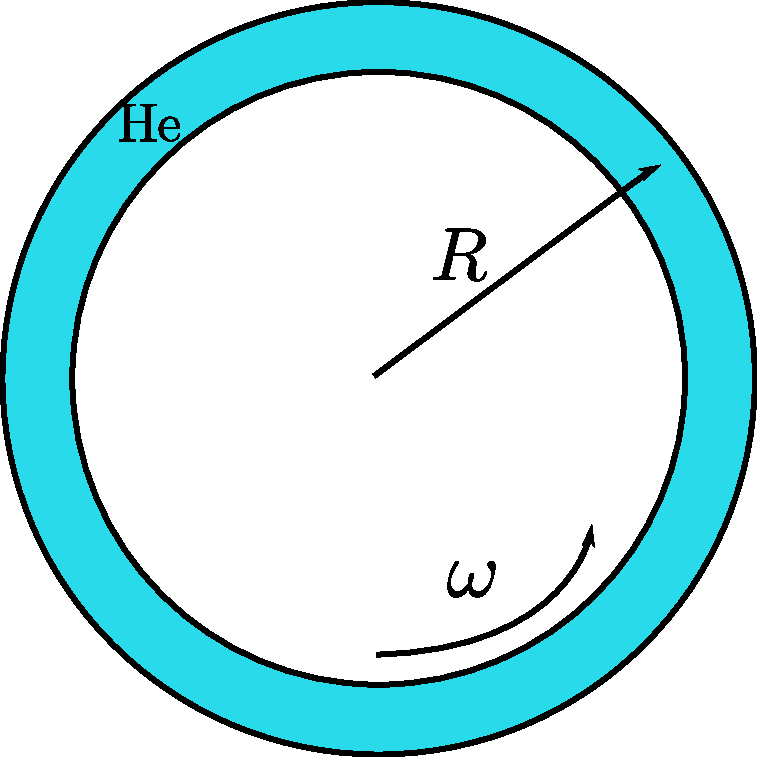
\includegraphics[width=.5\linewidth]{torus}
  \caption{
    % 
    The multiply connected toroidal geometry, of radius $R$, used to
    showcase superfluid behaviour. The anullus, which contains ${}^4$He
    atoms, rotates at an angular velocity $\omega$.
    % 
  }\label{fig:torus}
\end{figure}
% 
Assuming the pipe of radius $R$ is filled with liquid helium, and
rotates with angular velocity $\omega$, one can then obtain the
(temperature-dependent) orbital angular momentum of the system $L(T)$
by minimizing the effective free energy~\cite{leggett2006quantum}
%
\begin{equation}\label{eq:HF-angularmom}
  L(T) = I\left[f_n(T)\omega + f_s(T)n_w\omega_0\right]
\end{equation}
% 
Apart from the already defined quantities, we have introduced the
moment of inertia $I = N_0mR^2$, and defined the quantum unit of
angular velocity, $\omega_0 \equiv \hbar/(mR^2)$. Finally, $n_w$ is the
nearest integer to $\omega/\omega_0$, expressed as
%
\begin{equation}\label{eq:nearest-integer}
  n_w = \text{int} \left[\frac{\omega}{\omega_0} + \frac{1}{2}\right]
\end{equation}
% 
One needs to compare Eq.~\eqref{eq:HF-angularmom} with the angular
momentum of a normal liquid under the same circumstances, which is
given by $L = I \omega = N_0 \hbar \omega/\omega_0$. Keeping this in
mind, we can now introduce the two qualitatively different
experiments.


\paragraph{Persistent currents}
%
% protocol
%
The first experiment starts by rotating the torus at a large angular
velocity $\Omega \gg \omega_0$, on the high-temperature side of the
$\lambda$-point. Once the fluid equilibrates with the motion of the
container walls, we then cool the system through $T_{\lambda}$,
maintaining the same angular velocity $\Omega$. Finally, we stop the
container from rotating, and measure the angular momentum.
%
% observation
%
After a short while, proportional to the viscosity of the normal
component, its velocity $\bm{v}_n$ becomes zero. However, the
superfluid part of the liquid experiences no friction with the pipe
walls, and will therefore continue circulating indefinately! Since we
are not dealing with the ground state of the system, but with an
excited state with astronomical lifetime, we call this phenomenon
\textit{metastability of supercurrents} (``persistent currents'' is
another commonly found term).
%
% explanation
%
However, metastability of superflow is not a direct consequence of the
BEC state -- the underlying mechanism is one of topological origin:
consider the contour $C$ in Eq.~\eqref{eq:feynman} to run around the
torus of Fig.~\ref{fig:torus}. The current in the ring will be
proportional to the circulation Eq.~\eqref{eq:feynman}. Since the
latter is quantized, the windinding number $n_w$ is conserved, hence
so is the (super)current!
%
% vortices
%
Similar arguments explain the existence of so-called topological
defects in superfluid systems. Such defects are singularities of the
condensate wavefunction, for instance, vortex lines (or rings, if the
line closes in on itself) associated with the superfluid
component. The conservation laws presented above make the vortex a
highly stable configuration, as opposed to the case of a normal fluid,
where it is short-lived. In this sense, the circulating currents which
constitute the vortex are "persistent", corresponding to metastable
supercurrents. Furthermoe, a superfluid system cannot sustain bulk
vorticity due to Eq.~\eqref{eq:vorticity}, and the vortices are
quantized according to Eq.~\eqref{eq:feynman}.

In the final state with the container at rest, $\omega = 0$, so the
first term of Eq.~\eqref{eq:HF-angularmom} dissapears. The second term
survives, as the system cannot change its winding number. In the limit
of large $n_w$ the angular momentum will then be approximately given
by $L(T) \simeq f_s(T) I \Omega$. We see that one can reversibly
increase (or decrease) the angular momentum $L$ by varying the
temperature (provided, of course, that it is always kept below
$T_{\lambda}$).
%
% Landau criterion
%
Since the superfluid circulates despite any roughness of the container
walls, we can reasonably expect that an object moving though a
stationary fluid also experiences reduced friction. This led to a
series of experiments with charged ions being accelerated at various
speeds by an applied external electric field~\cite{Meyer1961,
  Allum1977}. It was seen that, in accordance with the Landau
criterion presented in Sec.~\ref{sec:cherenkov-emission}, there exists
a critical speed below which the ions experience reduced viscosity
(and actually no viscosity at all in the $T=0$ limit).



\paragraph{HF effect}
We now turn to the second experiment, which is arguably one of the
fundamental defining properties of superfluidity. The effect was first
predicted by Fritz London and then observed by G. Hess and W. Fairbank
in 1967 in the context of liquid helium, hence the name Hess-Fairbank
(HF) effect.
%
% protocol
%
As before, we cool the sample while rotating with a lower angular
velocity $\omega \ll \Omega$. We wait for the system to equilibrate,
and then measure the angular momentum, this time without stopping the
rotation of the container.
%
% observation
%
The value of $L$ will be given by Eq.~\eqref{eq:HF-angularmom},
instead of the classical $I \omega$ (that is why the HF effect is also
called nonclassical rotational inertia, NCRI).
%
We can now distinguish two different regimes. The first one, for
$\omega < \frac{1}{2}\omega_0$, implies $n_w = 0$, therefore
$L(T) = f_n(T)I\omega$, so the superfluid component contributes
nothing to the current. At $T=0$, $f_n(T) \rightarrow 0$ and we get
the spectacular result that the liquid completely ceases to rotate
along with the container!
%
In the general case, the second term of Eq.~\eqref{eq:HF-angularmom}
survives. If we again consider the zero-temperature limit, and plot
the angular momentum $L(0) = I\omega_0 n_w$ versus angular velocity
$\omega \geq \frac{1}{2}\omega_0$, we get a series of plateaus of
width $\omega_0$ at positions
$L = N_0 \hbar n_w = N_0 \hbar,\, 2N_0 \hbar$, and so on. The centers
of these plateaus all fall on the ``classical'' line
$L = N_0\hbar \omega/\omega_0$.
%
% explanation
%
A hand-waving explanation, for the simplest case of a noninteracting
atomic gas, goes as follows. In a noncondensed system rotating with
angular velocity $\omega$, the effective single-particle energies are
shifted by an amount $\hbar\omega \ell_{n_w}$, with $\ell_{n_w}$ the
angular momentum quantum number of state $n_w$. The Bose-Einstein
function then redistributes the particles to accomodate this shift,
producing a ``classical'' angular momentum. In a BEC however, all
$N_0$ atoms must be in the same state $n_w$, and posess the same value
of $\ell_{n_w}$. Their only allowed contribution to $L$ is then
$N_0(n_w\hbar)$. For small $\omega$, the condensate is in the
$n_w = 0$ state, and so it does not rotate with the container! This
argument can be formalized, so one can show the HF effect to be
impossible inside the framework of classical statistical mechanics,
much like the Bohr-Van Leeuwen theorem shows magnetism to be a purely
quantum phenomenon. Note that, while the HF effect can be (at least
hand-wavingly) explained without including interactions, these are
crucial to any theory of metastable currents.


\paragraph{Meissner effect}
As already explained in the introductory paragraph of this Section,
there is a deep underlying connection between superfluidity in a
neutral system and superconductivity in a charged one. In fact, the
analog of the HF effect in a charged system is the well-known Meissner
effect.
%
We now consider the same topology of Fig.~\ref{fig:torus}, and replace
the container by a crystal lattice and the liquid helium (or atomic
gas for that matter) by the electrons inside this lattice. If we now
keep the crystal at rest and produce a tangential vector potential
$\bm{A}(\rv) = A\hat{\phi}$, this will generate a flux
$\Phi = \oint \bm{A}(\rv)\cdot d\bm{l}$ inside the conducting ring
(usually called an ``Aharonov-Bohm''
flux). The definition of the ``superfluid''
velocity Eq.~\eqref{eq:supervelocity} now needs to be revised
according to the gauge-coupling recipe, which consists of replacing
the canonical momentum $\bm{p}$ by the kinematic one:
$\bm{p} \rightarrow \bm{p} - e\bm{A}(\rv)$. As a result, we get
%
\begin{equation}\label{eq:superconducting-velocity}
  \bm{v}_s(\rv) = \frac{1}{2m}\left(\bm{\nabla}\theta(\rv) -
    2e\bm{A}(\rv)\right)
\end{equation}
% 
where the factors of 2 appear because the macroscopic wavefunction is
now that of the center of mass of a Cooper-pair of electrons, so $m$
and $e$ are both multiplied by 2. The resulting Onsager-Feynman
quantization Eq.~\eqref{eq:feynman} then becomes
%
\begin{equation}\label{eq:superconducting-feynman}
  \oint_C \bm{v}_s(\rv) \cdot d\bm{l} = \frac{\hbar}{2m} \left(2\pi n_w -
    \frac{\Phi}{\Phi_0}\right)
\end{equation}
% 
where $\Phi_0 \equiv h/(2e)$ is the \textit{superconducting flux
  quantum}. If the (mass) supercurrent is given, as before, by
$\bm{j}_s = \rho_s \bm{v}_s$, then this new quantization condition
results in a non-zero current even for $n_w = 0$. Indeed, for
$\Phi < \frac{1}{2} \Phi_0$ (compare to the regime
$\omega < \frac{1}{2}\omega_0$ discussed for the HF effect), the
$n_w = 0$ state is realized and the electrical current $\bm{j}_e$ is
given by
%
\begin{equation}\label{eq:diamagnet}
  \bm{j}_e(\rv) = \frac{2e}{2m}\bm{j}_s = - \frac{e^2}{m^2}\rho_s(T) \bm{A}(\rv)
\end{equation}
%
This proves that, while in a normal conductor the flux $\Phi$ would
not generate any circulating current, a superconducting ring would
respond with a diamagnetic (note the minus sign in
Eq.~\eqref{eq:diamagnet}) electrical current proportional\footnote{The
  proportionality constant is called the susceptibility.} to the
vector potential $\bm{A}$. Coupling this with Maxwell's equations
immediately results in the well-known Meissner effect, namely the
expulsion of an applied magnetic field inside a superconducting
sample.


\paragraph{Synthetic gauge field}
We now proceed to a closer analysis of the connection between the
charged and neutral case. The Hamiltonian $H$ for a particle of charge
$q$ and mass $m$, moving in a vector potential $\bm{A}$, and in the
presence of an external potential $V$, is given by
Eq.~\eqref{eq:charged-ham}. In our problem, $V$ is imposed by the
toroidal geometry of the container, which is for now assumed to be
stationary in the inertial frame of the stars. On the other hand, the
Hamiltonian $H^{\prime}$, of a neutral particle with the same mass,
but this time in the frame that rotates with the container at an
angular velocity $\bm{\omega} = \omega\hat{z}$ is shown in
Eq.~\eqref{eq:neutral-ham},
%
\begin{align}
    H  = \frac{1}{2m}(\bm{p} - q\bm{A}(\rv))^2 & + V(\rv)\label{eq:charged-ham}\\
    H^{\prime}  = \frac{1}{2m}(\bm{p}^{\prime}-m\bm{\omega}\times
    \rv^{\prime})^2 & + V(\rv^{\prime}) - \frac{1}{2}m(\bm{\omega}\times
    \rv^{\prime})^2\label{eq:neutral-ham}
\end{align}
%
with $\rv^{\prime}$ being the coordinate (and $\bm{p}^{\prime}$ the
canonical momentum) in the rotating frame. Making use of the
cylindrical symmetry, one can decompose $\rv$ as $(r,\,z,\,\theta)$,
and therefore $\rv^{\prime} = (r,\,z,\,\theta-\omega t)$.
%
We now see that a neutral system in the rotating frame, apart from a
centrifugal term $- \frac{1}{2}m(\bm{\omega}\times \rv^{\prime})^2$,
is formally identical to a charged system in the rest frame, with the
correspondence $q\bm{A}(\rv) \leftrightarrow m\bm{\omega}\times
\rv$. This connection can be used to make a neutral particle
experience an ``effective'' electromagnetic vector potential. Its
gauge-coupling to this potential is what eventually led to the
celebrated concept of \textit{synthetic gauge field}.
%
In fact, such artificial, rotation-induced, gauge fields have already
been proposed in the context of ultracold atomic gases, in order to
asess their normal and superfluid
fractions~\cite{Cooper2010,Carusotto2011,John2011}.


\paragraph{BEC Experiments}
%
\begin{figure}[tb]\centering
  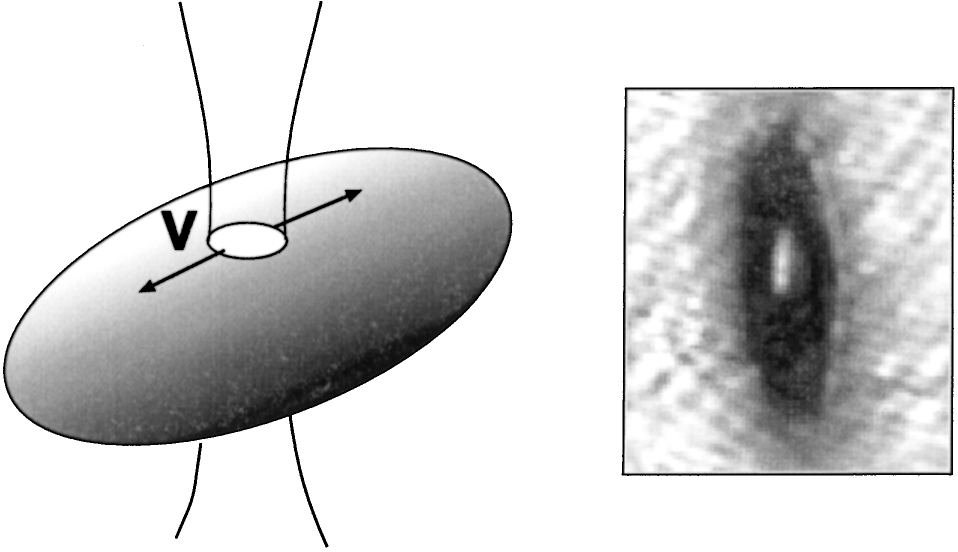
\includegraphics[width=.8\linewidth]{hole}
  \caption{
    % 
    Scanning a blue-detuned laser beam with velocity $v$, though the
    cigar-shaped atomic condensate (left panel), creates a density hole
    (right panel) larger than the healing length. The friction acting on
    this hole can then be used to asess the Landau critical velocity. From
    Ref.~\cite{Raman_1999}.
    % 
  }\label{fig:hole}
\end{figure}
% 
This naturally leads us to the topic of experimental evidence for
superfluid behaviour. The answer, however, will not be a clear-cut
one, as we have seen that it actually depends on which aspects of
superfluidity one is interested in, such as NCRI, persistent currents,
quantized vortices or reduced friction on impurities. Historically,
liquid ${}^4$He-II was the default system for exploring such physics,
however, new systems such as ultracold gases and, more recently,
microcavity polaritons (the subject of Chapter~\ref{cha:polaritons})
have also entered the picture. In the case of liquid helium,
superfluidity is relatively easy to detect, while BEC can only be
asessed through circumstantial evidence (such as neutron scattering),
as strong interactions oppose any large density changes. Ultracold
gases, on the other hand, present a spectacular BEC onset that can be
observed in the density profile, while superfluidity proves somewhat
more mysterious.
%
Regarding metastable supercurrents in a simply connected geometry,
Chevy and coworkers~\cite{Chevy2000} succeded in stirring an atomic
condensate, and then measuring its angular momentum using the
precession of certain collective modes.  Other studies were also shown
to produce a metastable single-vortex state (and even vortex lattices)
that persist, despite not being the ground state of the system (in
fact, it can be shown that the atomic BEC ground state is
characterised by the absence of any macroscopic current flow).
Interferometric measurements are commonly employed to see the
circulation around these vortex cores.  However, the lifetime of the
vortices is limited by how long it takes before they escape the
magnetic trap. To circumvent this limitation, persistent currents in
multiply connected geometries (such as toroidal traps) were also
investigated, for instance in Refs.~\cite{Ryu2007}
and~\cite{Ramanathan2011}.
% 
As far as the Landau criterion is concerned, an experiment similar to
the one accelerating charged ions through liquid helium was reported
in Ref.~\cite{Chikkatur_2000}. The authors used a Raman laser to
transfer a fraction of the condensed atoms into a different
(hyperfine) state. As a result, those atoms no longer experienced any
magnetic trapping, but only the effect of gravity. The mobility of the
free-falling atoms was then computed, revealing information about the
friction~\cite{Astrakharchik_2004} acting on them.  A fairly sharp
transition with a sudden increase in friction was observed, at
velocities close to the local speed of sound.
%
In the opposite limit of macroscopic ``impurities'' (large compared to
the healing length), Ref.~\cite{Onofrio_2000} details the use of a
blue-detuned laser beam, in order to create a density hole which is
then moved around the atomic condensate (see Fig.~\ref{fig:hole}).  By
measuring the density difference immediately ahead and behind the
hole, one can deduce the frictional force acting on it (see
Appendix~\ref{app:field-theory}). This experiment resulted in a
critical velocity about ten times smaller than the speed of sound,
presumably due to vortex creation by the macroscopic defect.


\section{Optical lattices}
\label{sec:optical-lattice}

\paragraph{Laser trapping}
An electric dipole moment $\bm{\mathcal{P}}$ placed in an external
electric field $\bm{\mathcal{E}}(\rv)$ aquires an energy
$\mathcal{V}(\rv) = -\bm{\mathcal{P}}\cdot \bm{\mathcal{E}}(\rv)$. If
an atom is placed in a light field, the oscillating electric field of
the latter induces an electric dipole moment
$\bm{\mathcal{P}} = \alpha \epsilon_0 \bm{\mathcal{E}}$ on the atom,
with $\epsilon_0$ the free-space permittivity and $\alpha$ the atomic
polarizability~\cite{feynman1979lectures}. Integrating, we obtain the
interaction energy of the atom with the field as
$\mathcal{V}(\rv) = -\frac{1}{2}\alpha \epsilon_0
\mathcal{E}^2(\rv)$. A classical model of the atom as a conducting
sphere of radius $r$ yields a polarizability of $4\pi r^3$. In
practice however, atomic transitions complicate this simple picture,
as the polarizability $\alpha$ depends on the driving frequency of the
light field. In the framework of the Drude
model~\cite{ziman1972principles}, one has
%
\begin{equation}\label{eq:polarizability}
  \alpha(\omega) = \frac{\alpha(0)\omega_0^2}{\omega_0^2 - \omega^2 - i \frac{\omega}{\tau}}
\end{equation}
% 
with the resonant frequency $\omega_0$, damping time $\tau$ and
$\alpha(0) > 0$ the static polarizability. The frequency-dependent
interaction energy $\mathcal{V}(\omega)$ thus obtained is sometimes
called the \textit{ac Stark effect}~\cite{Cohen-Tannoudji:101392}. If
the light frequency is smaller than that of the atomic resonance
$\omega < \omega_0$, the induced dipole is in phase with the electric
field, as $\Re[\alpha(\omega)] > 0$, and the force on the atom will
point in the direction of the square-field maxima (the situation is of
course reversed if instead $\omega > \omega_0$). This effect was first
used in Ref.~\cite{PhysRevLett.80.2027} to trap a BEC of sodium atoms
using a focused infrared laser beam (the dominant transition of Na is
the familiar $s \rightarrow p$ yellow emission). Interestingly, the
same physics can be used to create an optical lattice, as explained
below.

\paragraph{Optical lattice}
Consider a (plane wave) laser beam propagating along the $x$ axis,
with an associated electric field
$\bm{\mathcal{E}}(x,t) = \bm{\mathcal{E}}_0 \cos (k_x x - \omega t)$,
which reflects from a mirror situated at $x=0$. The interference
between the reflected and original beam produces a standing wave
$\bm{\mathcal{E}}_0[\cos(k_x x - \omega t) - \cos(k_x x + \omega t)]$,
with an intensity
$\abs{\mathcal{E}(x,t)}^2 = 4 \abs{\mathcal{E}_0}^2 \sin^2(k_x
x)\sin^2(\omega t)$. This results in an effective periodic lattice for
the atoms, with lattice spacing $b = \lambda_x/2$, where
$\lambda_x = 2\pi/k_x$. Such a one-dimensional lattice was first
demonstrated in Ref.~\cite{Anderson1686}. By tuning the strength of
the laser field, one can adjust the lattice depth, and by changing the
laser wavelength, one can modify the lattice constant. Adding more
laser beams can produce two- or even three-dimensional lattices, in a
variety of different geometries. For example, the simplest way to
create a 2D square lattice would be to superimpose a second lattice in
the $\hat{\bm{y}}$ direction, producing an optical potential of depth
$V_0$:
%
\begin{equation}\label{eq:square-potential}
  \mathcal{V}(x,y) = V_0[\sin^2(\pi x/b) + \sin^2(\pi y/b)]
\end{equation}
% 
The beam along $y$ should be orthogonally polarized with respect to
the one along $x$, in order to avoid interference effects.

\paragraph{Band structure}
The eigen-problem of a particle moving in a periodic potential given
by Eq.~\eqref{eq:square-potential} is well-known in the context of
solid-state band theory~\cite{ziman1972principles}, as the electrons
inside a solid also move in such a potential, produced in that case by
the crystal ions. The energy eigenstates are the Bloch waves
$\psi_{\gamma,\kv}(\rv) = e^{i\kv\cdot\rv} u_{\gamma,\kv}(\rv)$, where
$\hbar \kv$ is the \textit{quasimomentum}, restricted to the first
Brillouin zone (BZ)
$\left(-\frac{\pi}{b}, \frac{\pi}{b}\right) \times
\left(-\frac{\pi}{b}, \frac{\pi}{b}\right)$ and $\gamma = 0,1,\dots$
represents the \textit{band index}. The functions
$u_{\gamma,\kv}(\rv)$ are periodic in both the $\hat{\bm{x}}$ and
$\hat{\bm{y}}$ direction, with period $b$. To see how these bands
arise, one can expand both the wavefunction $\psi_{\gamma,\kv}$ as
well as the potential $\mathcal{V}$ in a Fourier series, making use of
their periodicity. Inserting this expansion into the time-independent
Schr\"odinger equation, we get a linear system of equations for the
Fourier coefficients. For fixed $\kv$, we obtain
different\footnote{Truncating the Fourier expansion to a finite number
  of terms $n$ results in $2n+1$ bands.} eigenenergies,
$E_{\gamma}(\kv)$. These eigenenergies form bands (called \text{Bloch
  bands}) when $\kv$ is varied inside the BZ. Each band as a certain
width in energy (unsurprisingly called the bandwidth) and consecutive
bands are separated by gaps, meaning certain energies are not
allowed. Furthermore, each eigenenergy has an associated
eigenfunction, completely determined by the set of Fourier
coefficients with index $\gamma$. The solution of course depends on
the value of $V_0$, and we can distinguish two limiting cases,
depending on the ratio of the bandwidths to the energy gaps. In the
weak-potential limit, the bandgaps are much smaller than the
bandwidths, and the eigenenergies have a pronounced dependence on
quasimomentum. The opposite limit, which is the one we want to focus
on, is the regime of deep lattices, also called the
\textit{tight-binding} (TB) limit. The band dispersion is now flatter
compared to the previous case, and the bandwidth/gap ratio is much
smaller.

\paragraph{Tight binding}
For low temperatures in the TB limit, only the lowest energy band
$\gamma = 0$ is occupied, so we subsequently drop the band
index. Since the potential wells are so deep, the lowest band is
adequately described by considering localized wavefunctions at each
well, i.e. at the minima of Eq.~\eqref{eq:square-potential}. Suppose
now that a function $w(\rv)$ exists such that the Bloch waves are
given by
%
\begin{equation}\label{eq:wanier}
  \psi_{\kv} (\rv) = \mathcal{N} \sum_{m,n} e^{i\kv \cdot \rv_{m,n}} w(\rv - \rv_{m,n})
\end{equation}
% 
where $\mathcal{N}$ is a normalization factor and
$\bm{r}_{m,n} = m b \hat{\bm{x}} + n b \hat{\bm{y}}$ are the well
positions. Eq.~\eqref{eq:wanier} represents a wave,
$e^{i\kv \cdot \rv_{m,n}}$, whose phase and amplitude at each well is
given by the localized function $w$, called the \textit{Wannier
  function}~\cite{ziman1972principles}. It can be shown that Wannier
functions centered at different wells are orthogonal to each other and
form a complete basis. The Wannier functions are thus a unitary
transformation of the Bloch functions, suitable for the case when
particle dynamics is described by inter-well tunneling (hopping)
between nearest-neighbour wells. 

In the case of a BEC, when the number of ultracold atoms per lattice
well is small, the ``discrete structure'' of the condensate becomes
relevant and we must replace the GP description Eq.~\eqref{eq:TDGP} we
have used so far with a lattice model, such as the Bose-Hubbard
model~\cite{PhysRevB.40.546}, as suggested in
Ref.~\cite{Jaksch3108}. For a condensate confined in the optical
potential Eq.~\eqref{eq:square-potential}, with an additional harmonic
trap $U(\rv)$, the spinless Bose-Hubbard Hamiltonian in 2D can be
written as~\cite{zwerger2003}
%
\begin{equation}\label{eq:BH-ham}
  \mathcal{H}\sub{BH} = \mathcal{H}_0 + \frac{U}{2}\sum_{m,n} \hat{n}_{m,n}(\hat{n}_{m,n} - 1) + \sum_{m,n} \epsilon_{m,n} \hat{n}_{m,n}
\end{equation}
% 
where $U \propto g$ is the on-site interaction strength and
$\epsilon_{m,n} \propto U(\rv_{m,n})$ is the energy offset due to the
harmonic trap. Futhermore,
$\hat{n}_{m,n} = \hat{a}_{m,n}^{\dagger} \hat{a}_{m,n}$ denotes the
number operator for site $(m,n)$ and $\hat{a}_{m,n}^{\dagger}$
($\hat{a}_{m,n}$) is the bosonic creation (destruction) operator for
that site. Finally, the kinetic part
%
\begin{equation}\label{eq:kinetic-part}
  \mathcal{H}_0 = -J \sum_{m,n} \left(\hat{a}^{\dagger}_{m+1,n}\hat{a}_{m,n} + \hat{a}^{\dagger}_{m,n+1}\hat{a}_{m,n}\right) + \text{H.c.}
\end{equation}
% 
can be diagonalized to yield the Bloch dispersion
%
\begin{equation}\label{eq:tb-dispersion}
  E(\kv) = -2J\left[\cos(k_x b) + \cos(k_y b)\right]
\end{equation}
% 
where the tunneling amplitude $J$ is an exponentially decreasing
function of $V_0$~\cite{zwerger2003}. The characteristic tunneling
energy scale is given by the bandwidth, which in this case is $8J$.

Hamiltonian Eq.~\eqref{eq:BH-ham} supports a zero-temperature quantum
phase transition between a superfluid and a Mott-insulating phase, at
a critical value of the ratio $U/J$. This transition was
experimentally observed for the case of a bosonic BEC in a 3D optical
lattice, as reported in Ref.~\cite{greiner2002quantum}. Increasing the
lattice depth $V_0$, the authors went from a gapless, superfluid
regime dominated by the kinetic term Eq.~\eqref{eq:kinetic-part} to a
gapped Mott-insulator state, where the atoms are localized and the
on-site interaction term in Eq.~\eqref{eq:BH-ham} is dominant.

\section{Harper-Hofstadter model}
\label{sec:hh-atoms}
\paragraph{Landau levels}
In Sec.~\ref{sec:optical-lattice} we introduced the quantized Bloch
bands, characterising particles in a periodic potential. A similar
quantization also occurs in the case of a charged particle moving
perpendicular to a constant uniform magnetic field, and the allowed
energy bands are called \textit{Landau
  levels}~\cite{Landau:101810}. In a magnetic field
$\bm{B} = B \hat{\bm{z}}$, the relevant energy and length scales for a
particle with charge $e$ and mass $m$ are set by the \textit{cyclotron
  frequency} $\omega_c = eB/m$ and \textit{magnetic length}
$l\sub{m} = \sqrt{\hbar/eB}$, respectively. In this Section we want to
explore the fate of the Bloch bands in presence of a magnetic
field. Alternatively, one could also start from a Landau quantized
system and perturb it via a weak periodic
potential~\cite{PhysRev.180.633,PhysRevB.46.12606}, the two approaches
having distinct validity ranges.

\paragraph{Hofstadter butterfly}
One of the simplest TB models for Bloch electrons in uniform magnetic
fields is the \textit{Harper-Hofstadter
  model}~\cite{harper1955magnetic,hofstadter1976butterfly}. Its
relevant dimensionless parameter is the ratio of flux $\Phi$ through a
lattice cell to one \textit{Dirac flux quantum}\footnote{As opposed to
  the superconducting flux quantum of Sec.~\ref{sec:superfluid-atom}.}
$\Phi_0=h/e$
%
\begin{equation}\label{eq:alpha}
  \alpha = \frac{\Phi}{\Phi_0} = \frac{eBb^2}{h}
\end{equation}
% 
Physically, $\alpha$ reflects\footnote{Not to be confused with the
  atomic polarizability, also denoted by $\alpha$.} the
commensurability of the lattice period $b$ and the magnetic length
$l\sub{m}$, as it can be recast in the form
$\alpha = \frac{1}{2\pi}\left(b/l\sub{m}\right)^2$.  The resulting
single-particle energy spectrum of the model depends on the
rationality of $\alpha$. If $\alpha = p/q$, for $p$ and $q$ co-prime
integers, the Bloch band splits into $q$ distinct magnetic
subbands. For $\alpha$ irrational, the spectrum consists instead of an
infinite number of energy levels, forming a Cantor set. The union of
all allowed energies as a function of $\alpha$ forms a self-similar
fractal, shown in Fig.~\ref{fig:butterfly} and known as
\textit{Hofstadter’s butterfly}~\cite{hofstadter1976butterfly}. In the
continuum limit ($b \rightarrow 0$, with fixed $B$), $\alpha \ll 1$
and the bands group into clusters that can be identified with the
Landau fan predicted in the absence of a lattice potential.
%
\begin{figure}[tb]\centering
  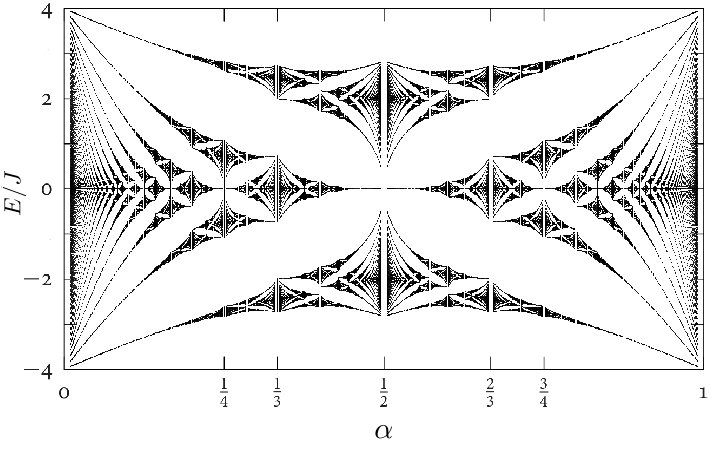
\includegraphics[width=\linewidth]{hhbutterfly}
  \caption{
    % 
    Hofstadter's butterfly, representing the internal structure of the
    lowest Bloch band in a uniform magnetic field. For rational values of $\alpha
    = p/q$, the spectrum has $q$ magnetic subbands, which become
    increasingly narrow as $q$ gets larger. Adapted from
    Ref.~\cite{hofstadter1976butterfly}.
    % 
  }\label{fig:butterfly}
\end{figure}
% 

\paragraph{HH experiments}
Solid-state experiments in the Hofstadter regime are notoriously
difficult, since the inter-atomic spacing of a crystal lattice is a
few {\AA}ngstr\"oms, and achieving a comparable magnetic length would
require a field of about $10^4$ Tesla. Signatures of the Hofstadter
bands have instead been seen in artificial superlattices with
periodicities of tens of
nanometers~\cite{dean2013hofstadter,yu2014hierarchy}. In the context
of neutral ultracold atoms, synthetic gauge potentials paved the way
for the exploration of similar
physics~\cite{dalibardrmp2011,goldman_repprog_2014}. For instance,
rotating a harmonically trapped condensate with a high angular
velocity (comparable to the radial trap frequency) allowed BEC
experiments~\cite{PhysRevLett.92.040404} to enter the lowest Landau
level (LLL) regime. Rotating 2D optical lattices have also been
realized~\cite{PhysRevLett.104.050404}, but the first implementation
of the Harper-Hofstadter (HH) model with ultracold
atoms~\cite{aidelsburger2013hh,miyake2013hh} employed a different
method~\cite{goldman_repprog_2014} of generating the artificial
magnetic field, namely \textit{laser-assisted
  tunneling}~\cite{1367-2630-5-1-356} based on a linear superlattice
potential~\cite{1367-2630-12-3-033007}. In a nutshell, tunneling
between lattice sites required atoms to absorb and emit photons
produced by external lasers. The interaction with said lasers
generated a net phase change equivalent to the flux of a magnetic
field. The total phase accumulated by an atom when performing a loop
around a lattice cell (plaquette) was $\sim \pi/2$ in these
experiments.

\paragraph{Aharonov-Bohm phase}
In quantum mechanics, the phase of the wavefunction of a charged
particle moving between positions $\rv_1$ and $\rv_2$ is changed by
the presence of a magnetic field $\bm{B} = \bm{\nabla} \times \bm{A}$
by~\cite{feynman1979lectures}
%
\begin{equation}\label{eq:AB-phase}
  \phi_{12} = \frac{e}{\hbar}\int_{{\rv}_{1}}^{{\rv}_{2}} d\rv \cdot \bm{A}(\rv)
\end{equation}
% 
where the integral is taken along an oriented path from point ``1'' to
point ``2''. Therefore, $\phi_{21} = -\phi_{12}$ and, if we consider a
smooth closed integration contour $\mathcal{C}$ instead of two
separate points, the total phase change (or \textit{Aharonov-Bohm
  phase}) along $\mathcal{C}$ is
%
\begin{equation}\label{eq:AB-closed}
  \phi_{\mathcal{C}} = \frac{e}{\hbar}\int_{\mathcal{S}}
  d^2 \rv \cdot \bm{\nabla} \times
  \bm{A}(\rv) = 2\pi \frac{\Phi_B}{\Phi_0}
\end{equation}
% 
where $\Phi_B$ is the magnetic flux through a smooth surface
$\mathcal{S}$ bounded by the curve $\mathcal{C}$ with positive
orientation, according to Stoke's theorem.

\paragraph{Peierls phases}
On the 2D square lattice in Fig.~\ref{fig:hh-lattice}, one can define
the magnetic phases
$\phi_{m,n} = \left(\phi^{x}_{m,n},\phi^{y}_{m,n}\right)$ along the
$\hat{\bm{x}}$ and $\hat{\bm{y}}$ directions in a similar manner, as
%
\begin{figure}[tb]\centering
  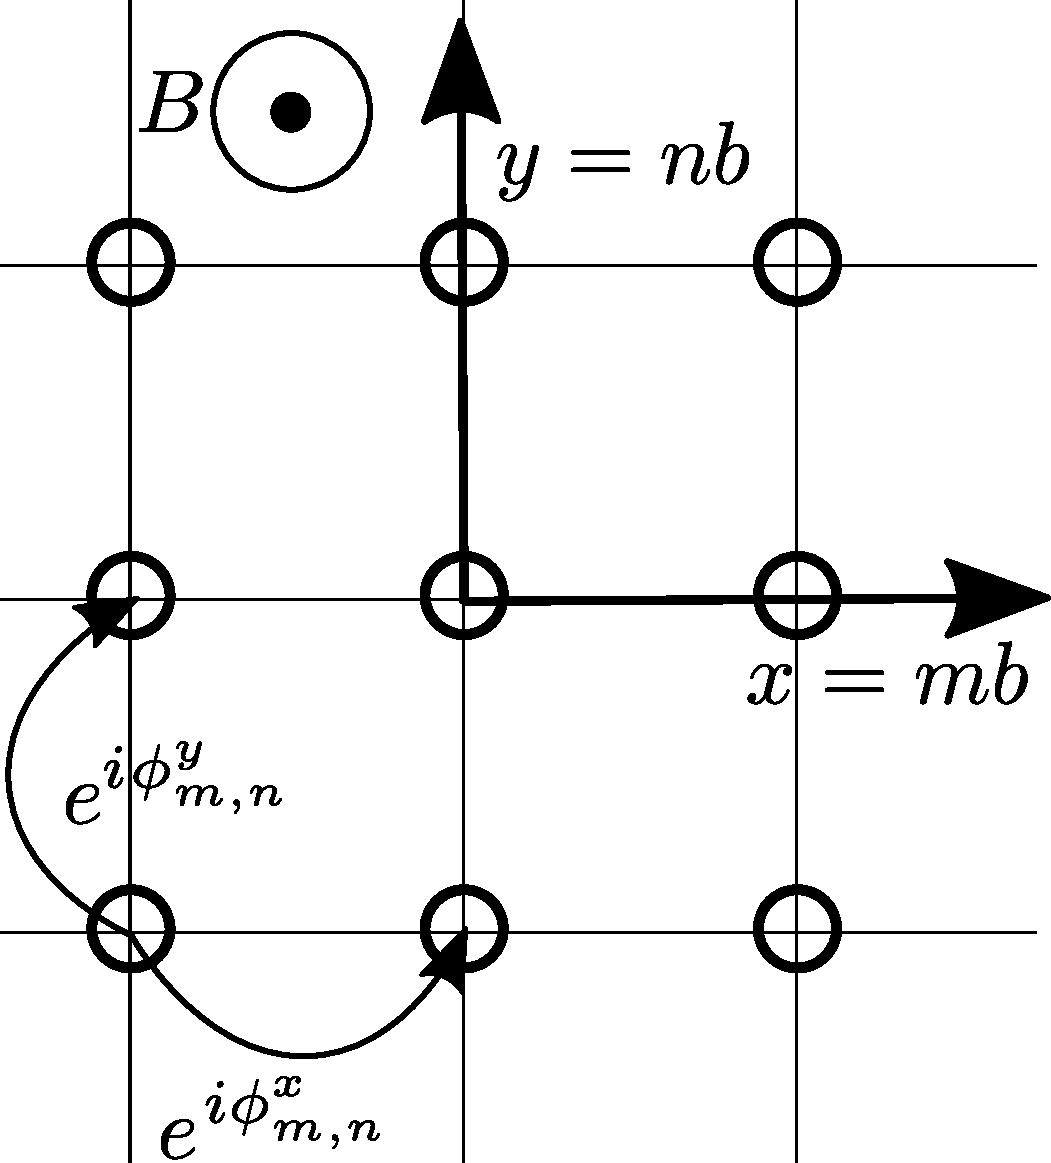
\includegraphics[width=.4\linewidth]{lattice}
  \caption{
    % 
    2D square lattice pierced by a homogeneous static magnetic field
    $\bm{B} = B\hat{\bm{z}}$. The lattice constant is $b$, and the curved
    arrows indicate the field-induced hopping phases.
    % 
  }\label{fig:hh-lattice}
\end{figure}
%
\begin{align}
  \phi^{x}_{m,n} &= \frac{e}{\hbar}\int_{{\rv}_{m,n}}^{{\rv}_{m+1,n}} d\rv \cdot \bm{A}(\rv) &
  \phi^{y}_{m,n} &= \frac{e}{\hbar}\int_{{\rv}_{m,n}}^{{\rv}_{m,n+1}} d\rv \cdot \bm{A}(\rv)
\end{align}
where the integrals are now taken along the links joining neighbouring
sites. Using Eq.~\eqref{eq:AB-closed}, the flux $\Phi$ through a
plaquette can be related to the total phase $\phi_{\square}$
accumulated on a contour enclosing the plaquette in a counterclockwise
sense
%
\begin{equation}\label{eq:lattice-curl}
  \phi_{\square} \equiv \sum_{\circlearrowleft
    \square} \phi_{m,n} =  \phi^x_{m,n} + \phi^y_{m+1,n} - \phi^x_{m,n+1} - \phi^y_{m,n} = 2\pi \alpha 
\end{equation}
% 
Note that $\phi_{\square}$ is gauge-independent, unlike the
\textit{Peierls phases} $\phi_{m,n}$.



\paragraph{HH Hamiltonian}
To obtain the HH Hamiltonian, we introduce a static uniform magnetic
field into the single-band Bose-Hubbard model Eq.~\eqref{eq:BH-ham} of
Sec.~\ref{sec:optical-lattice}. We follow Hofstadter's original
treatment, and neglect on-site interactions\footnote{For a treatment
  that includes interactions in the Bogoliubov approximation, see
  Ref.~\cite{PhysRevA.83.013612}.}, as well as the harmonic
trapping. The kinetic term Eq.~\eqref{eq:kinetic-part} is then
modified according to Peierls' substitution~\cite{peierls1933} to
include the hopping phases $\phi_{m,n}$
%
\begin{equation}\label{eq:HH-hamiltonian}
  \mathcal{H}_0 = -J \sum_{m,n} \left(e^{i\phi^x_{m,n}}\hat{a}^{\dagger}_{m+1,n}\hat{a}_{m,n} + e^{i\phi^{y}_{m,n}}\hat{a}^{\dagger}_{m,n+1}\hat{a}_{m,n}\right) + \text{H.c.}
\end{equation}
% 
These phases act to ``frustrate'' the hopping, such that for
noninteger $\alpha$ it is impossible to minimize the kinetic energy
simultaneously on all lattice links~\cite{moessner2001}. The
Hamiltonian is no longer invariant under translations by a single
lattice site in any direction, because fixing a gauge for the vector
potential $\bm{A}(\rv)$ reduces the physical symmetry of the
lattice. In fact, it can be shown~\cite{jain2007composite} that a
translation of $\bm{A}$ is equivalent to a gauge transformation,
suggesting that new translation operators that would commute with
Eq.~\eqref{eq:HH-hamiltonian} can be constructed as a combination of
translation and gauge transformation.


\paragraph{Magnetic translation operators}
We define the \textit{magnetic translation operators} (MTOs)
~\cite{zak1964group,zak1964representations} as

%
\begin{align}
  \tx &= \sum_{m,n} \hat{a}^{\dagger}_{m+1,n}\hat{a}_{m,n}e^{i\theta^x_{m,n}} &
  \ty &= \sum_{m,n} \hat{a}^{\dagger}_{m,n+1}\hat{a}_{m,n}e^{i\theta^y_{m,n}}
\end{align}
%
where the phases $\theta_{m,n}$ are to be determined by imposing
$\left[\hat{T}, \mathcal{H}_0 \right] = 0$, leading
to~\cite{bernevig2013topological}
%
\begin{align}
  \theta^x_{m,n} &= \phi^x_{m,n} + 2\pi\alpha n &
  \theta^y_{m,n} &= \phi^y_{m,n} - 2\pi\alpha m 
\end{align}
% 
While the specific form of the MTOs depends on the choice of gauge,
their commutator is gauge independent
%
\begin{equation}\label{eq:TxTy}
  \tx \ty = \ty \tx  e^{i2\pi\alpha} 
\end{equation}
% 
and vanishes only if $\alpha$ is an integer, a situation equivalent to
the zero-field case. In order to proceed, we point out that
Eq.~\eqref{eq:TxTy} has a transparent physical interpretation. If we
act on the single-particle state
$\ket{m,n} = \hat{a}^{\dagger}_{m,n}\ket{0}$
%
\begin{equation}\label{eq:translation-loop}
  \ty^{\dagger} \tx^{\dagger} \ty \tx \ket{m,n} = e^{-i2\pi\alpha} \ket{m,n}
\end{equation}
%
we see that performing a counterclockwise loop around a unit cell
results in the accumulation of a phase proportional to the flux inside
the cell. This can be generalized to a macrocell containing
$r \times s$ original lattice cells, to deduce that
%
\begin{equation}
  \tx^r\ty^s = \ty^s\tx^re^{i(rs)2\pi\alpha}
\end{equation}
% 
For $\alpha = p/q$ the commutator $\left[\tx^r, \ty^s\right]$ vanishes
if $p (rs)/q$ is an integer. The smallest possible macrocell is given
by $rs = q$ and is called the \textit{magnetic unit cell}. For this
choice of unit cell, $\{\tx^r, \ty^s, \mathcal{H}_0\}$ form a complete
set of commuting operators, so we can find simultaneous eigenstates,
labeled by the quasimomentum $\hbar\kv^0$ which is now restricted to
the \textit{magnetic Brillouin zone} (MBZ)
$\left(-\frac{\pi}{rb}, \frac{\pi}{rb}\right) \times
\left(-\frac{\pi}{sb}, \frac{\pi}{sb}\right)$.


\paragraph{HH spectrum}
%
\begin{figure}[tb]\centering
  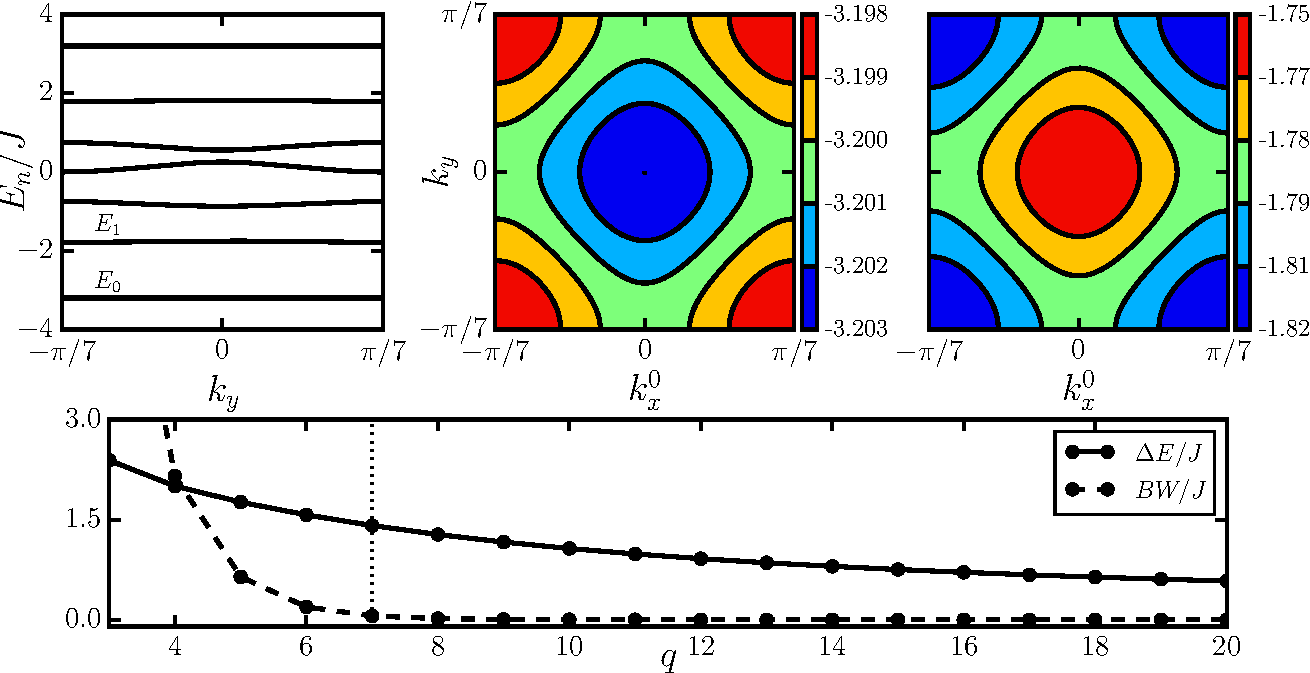
\includegraphics[width=\linewidth]{hhgapwidth}
  \caption{
    % 
    \emph{Top panels:} Single-particle energy spectrum (left)
    $E_n(k_x^0=0,k_y)$ of the HH Hamiltonian Eq.~\eqref{eq:HH-hamiltonian}
    for $\alpha = 1/7$ and dispersion of the two lowest bands, $E_0(\kv)$
    (middle) and $E_1(\kv)$ (right) in (part of) the MBZ.  \emph{Bottom
      panel:} Energy gap (continuous line) $\Delta E =
    \left<E_1(\vt{k})\right>_{\vt{k}} - \left<E_0(\vt{k})\right>_{\vt{k}}$
    (here $\left<\cdot\right>_{\vt{k}}$ denotes an average over the MBZ)
    and bandwidth of $E_0(\kv)$ (dashed line, $\times 10$) for $p =
    1$. The dotted vertical line marks the location of the $q = 7$ case
    shown above.
    % 
  }\label{fig:hh-energy-levels}
\end{figure}
% 
To obtain the spectrum of $\mathcal{H}_0$, we need to solve its
associated Schr\"odinger equation,
$\mathcal{H}_0\ket{\psi} = E\ket{\psi}$. We expand the eigenstates
$\ket{\psi}$ in the single-particle basis
$\ket{\psi} = \sum_{m,n} \psi_{m,n} \ket{m,n}$ and obtain an equation
for the coefficients $\psi_{m,n}$
%
\begin{multline}\label{eq:HH-schrodinger}
  -J \big(e^{-i\phi^x_{m,n}}\psi_{m+1,n}+e^{i\phi^x_{m-1,n}}\psi_{m-1,n}\\
  {} + e^{-i\phi^y_{m,n}}\psi_{m,n+1} + e^{i\phi^y_{m,n-1}}\psi_{m,n-1}\big) = E\psi_{m,n}
\end{multline}
% 
We fix the Landau gauge $\bm{A}(x,y)=Bx\hat{\bm{y}}$ for simplicity,
so $\phi_{m,n} = (0,2\pi\alpha m)$ and we choose the magnetic unit
cell\footnote{In the symmetric gauge, the magnetic unit cell is
  larger, containing $2q \times 2q$ sites.}
$r \times s = q \times 1$, for which the commuting MTOs read
%
\begin{align}
  \hat{T}^q_x &= \sum_{m,n} \hat{a}^{\dagger}_{m+q,n} \hat{a}_{m,n} &
  \hat{T}_y &= \sum_{m,n} \hat{a}^{\dagger}_{m,n+1} \hat{a}_{m,n}
\end{align}
%
justifying the plane wave ansatz\footnote{Here $k_y$ is defined in the
  full BZ.}  $\psi_{m,n} = e^{ik_ynb}e^{ik_x^0mb} \psi_m$ subject to
the periodic boundary conditions $\psi_{m+q} = \psi_m$. Substituting
this ansatz into Eq.~\eqref{eq:HH-schrodinger} yields the
\textit{Harper equation}~\cite{Harper_1955}
%
\begin{equation}\label{eq:Harper}
  -J\left[e^{-ik_x^0 b} \psi_{m-1} + 2\cos\left(k_yb - 2\pi\alpha m\right)\psi_m + e^{ik_x^0 b}\psi_{m+1}\right] = E\psi_m
\end{equation}
% 
Calculating the single-particle spectrum of
Eq.~\eqref{eq:HH-hamiltonian} is therefore equivalent to solving the
eigenvalue equation
$\sum_{m^{\prime}=0}^{q-1} H_{mm^{\prime}}\psi_{m^{\prime}} =
E\psi_m$, $m=0,\dots,q-1$ for the $q \times q$ matrix $H$ defined
as\footnote{If $q = 2$, $m+1 \bmod q = m-1 \bmod q$ and
  $H_{01} = H_{10} = -2J\cos (k_x^0b)$.}
%
\begin{equation}\label{eq:Hmatrix}
  H_{mm^{\prime}}(k_x^0,k_y) = -J\times\begin{cases}
    e^{-ik_x^0 b} & \text{if $m^{\prime} = m-1 \bmod q$}\\
    2\cos\left(k_yb - 2\pi\alpha m\right) & \text{if $m^{\prime} = m$}\\
    e^{ik_x^0 b}  & \text{if $m^{\prime} = m+1 \bmod q$}\\
    0 & \text{otherwise}
  \end{cases}
\end{equation}
%
For integer $\alpha$ we recover the lowest Bloch band
Eq.~\eqref{eq:tb-dispersion}, while for $\alpha = p/q$ this band
splits into $q$ bands with dispersion $E_n(k_x^0,k_y)$, $n =
0,\dots,q-1$. 

\paragraph{Spectrum discussion}
In the top-left panel of Fig.~\ref{fig:hh-energy-levels} we show an
example of the spectrum computed by diagonalizing $H$ for
$\alpha = 1/7$. The $E=0$ level is at the centre of the middle band,
and there are $q-1$ gaps separating the bands. For even values of $q$,
the spectrum is symmetric with respect to $E=0$ and the two central
bands touch at zero energy. Around these degeneracy points, the
dispersion is linear~\cite{PhysRevB.39.11943}, while in all other
cases it is quadratic near its minimum. The $\alpha=1/2$ case is
particularly interesting by analogy to graphene-related
physics~\cite{RevModPhys.81.109}, as there are two inequivalent
``Dirac points'' and the Hamiltonian preserves time-reversal
symmetry. Inspecting the middle and right panels we note that, despite
the reduced symmetry of $\mathcal{H}_0$, the dispersion has the full
$C_4$ rotational symmetry of the underlying square lattice. One can
formally define rotation and reflection operators which, together with
the MTOs, constitute the full \textit{projective symmetry
  group}~\cite{PhysRevB.65.165113}.  The bottom panel of
Fig.~\ref{fig:hh-energy-levels} shows the evolution of the lowest
energy gap $\Delta E$, as well as the bandwidth $BW$ of the lowest
band as function of $q$ (for the case $\alpha = 1/q$). The lowest band
gets flatter, as the continuum ($q \rightarrow \infty$) LLL
eigenstates are the solutions of the lowest band of the HH
model~\cite{bernevig2013topological}, and $\Delta E$ decreases like
$\sim 1/q$, as the number of gaps is $\sim q-1$ (excluding the band
bottom and band top).


\paragraph{HH topology}
The energy bands of the HH model are topologically nontrivial, as
characterized by their non-zero \textit{Chern numbers} -- topological
invariants that are linked to the quantization of the Hall
conductivity in the integer quantum Hall (QH)
effect~\cite{thouless}. In fact, solutions of the Harper equation
Eq.~\eqref{eq:Harper} were also studied in connection with the QH
effect~\cite{PhysRevB.39.11943}. We make use of these topological
properties in Chapter~\ref{cha:landau}, where we consider the HH model
in the presence of an external harmonic trap in a dissipative system.


\begin{subappendices}
\section{Conservation laws for the GP field}
\label{app:field-theory}
%
In this Appendix we use (classical) field theory to derive the
conservation laws associated with the time-dependent Gross-Pitaevskii
Eq.~\eqref{eq:TDGP}. We start by recasting the TDGP using Einstein's
summation convention, with the notation $\bm{x} \equiv (x_1, x_2,
x_3)$ and $\partial_k \equiv \frac{\partial}{\partial x_k}$ ($k =
1,2,3$)
%
\begin{equation}\label{eq:GP-field}
    i\hbar\partial_t\phi_0(\bm{x},t) = 
  \left[-\frac{\hbar^2}{2m}\partial_k\partial_k + U(\bm{x},t) + g N_0 |\phi_0(\bm{x},t)|^2\right]\phi_0(\bm{x},t)
\end{equation}
% 
This equation can be deduced by extremalization of the action
$S = \int dt \int d\bm{x} \,L$, where the Lagrangian density
$L = L[\p, \pa \p, \ps, \pa \ps, \xv, t]$ is given by
%
\begin{equation}\label{eq:GP-action}
  L = -N_0\left[\hbar \imag\left(\ps \pa_t \p\right) + 
\frac{\hbar^2}{2m}\pa_k\p\pa_k\ps + U\abs{\p}^2 + \frac{g}{2}N_0\abs{\p}^4 \right]
\end{equation}
% 
For compactness, let $x_4 = i c t$,\footnote{$c$ is the speed of
  light, but it is just a constant for our purposes, and will drop out
  from all final results.}  and we can define the canonical
energy-momentum tensor~\cite{Landau:101807}, following the usual
field-theory prescription~\cite{wentzel2003quantum}
%
\begin{equation}\label{eq:en-mom-tensor}
  T_{\mu \nu} = - \pa_{\nu} \p \frac{\pa L}{\pa (\pa_{\mu} \p)} - \pa_{\nu} \ps \frac{\pa L}{\pa (\pa_{\mu} \ps)} + L \delta_{\mu \nu}
\end{equation}
% 
where the indices $\mu,\,\nu$ run from 1 to 4. As the complex scalar
field $\ps$ (and $\p$) satisfy the Euler-Lagrange
equations~\cite{Landau:101804} resulting in Eq.~\eqref{eq:GP-field}
(and its complex conjugate), we have
%
\begin{equation}\label{eq:conservation-laws}
  \pa_{\mu} T_{\mu\nu} = \pa_{\nu} L
\end{equation}
% 
from which energy and momentum conservation immediately
follow.\footnote{Conservation of angular momentum imposes the
  additional requirement that $T_{\mu\nu} = T_{\nu\mu}$.}
%
To see this explicitly, we split the temporal and spatial parts of
Eq.~\eqref{eq:conservation-laws} to obtain
%
\begin{align}
  \pa_t T_{4 4} + i c \pa_{k} T_{k 4} & = \pa_t L\label{energy-cons}\\
  \pa_t T_{4 l} + i c \pa_{k} T_{k l} & = i c \pa_{l} L\label{mom-cons}
\end{align}
%
Direct subsitution into Eq.~\eqref{eq:en-mom-tensor} shows that
$T_{4 4} = -H$, where the energy density $H$ is given by
%
\begin{equation}\label{eq:en-density}
  H = N_0\left(
\frac{\hbar^2}{2m}\pa_k\p\pa_k\ps + U\abs{\p}^2 + \frac{g}{2}N_0\abs{\p}^4 \right)
\end{equation}
% 
while $T_{k 4} = \frac{i}{c}S_k$, with the energy flux density
%
\begin{equation}\label{eq:energy-source}
  S_k = -\frac{N_0\hbar^2}{m}\real\left(\pa_t\ps\pa_k\p\right)
\end{equation}
% 
Regarding Eq.~\eqref{mom-cons}, we get $T_{4 l} = i c J_l$, with the mass
current density (compare to Eq.~\eqref{eq:bec-current})
\begin{equation}\label{eq:current}
  J_l = N_0\hbar\imag\left(\ps \pa_l \p\right)
\end{equation}
and the momentum flux density tensor $\Pi_{kl} \equiv T_{kl}$
%
\begin{equation}
  \Pi_{kl} = \frac{N_0\hbar^2}{m}\real\left(\pa_l\ps\pa_k\p\right) + \delta_{kl}\left(\frac{g}{2}N_0^2\abs{\p}^4 -
    \frac{N_0\hbar^2}{4m}\pa_i\pa_i\abs{\p}^2\right)
\end{equation}
% 
Combining all the above, one can rewrite
Eq.~\eqref{eq:conservation-laws} as
%
\begin{align}
  \pa_t H + \pa_{k} S_k & = N_0\abs{\p}^2 \pa_{t} U\\
  \pa_t J_l  + \pa_{k} \Pi_{k l} & = -N_0\abs{\p}^2 \pa_{l} U\label{eq:mom-cons-pi}
\end{align}
%
We now focus on Eq.~\eqref{eq:mom-cons-pi}, which shows momentum
conservation. For a more transparent physical interpretation, one can
make use of the Madelung transformation Eq.~\eqref{eq:madelung} and
integrate over a volume $V$, obtaining
%
\begin{equation}\label{eq:gauss}
  \pa_t P_l  + \oint_S \Pi_{k l} \hat{n}_k d S  = -\int_{V}  \rho \pa_{l} U dV
\end{equation}
% 
where we made use of the divergence theorem for tensor
fields~\cite{the_brick} in order to express the volume integral as an
integral over the surface $S$ which encloses $V$. Here $\bm{\hat{n}}$
is the outward-pointing unit normal to $S$ at each point, and we also
introduced the total momentum of the field,
$\bm{P} = m \int_{V} \rho \bm{v}\, dV$ (with $\bm{v}$ the velocity
Eq.~\eqref{eq:supervelocity}). The hydrodynamic form of the momentum
flux density then reads
%
\begin{equation}\label{eq:pressure}
  \Pi_{k l} = \frac{\hbar^2}{4m\rho} \pa_k\rho \pa_l\rho + m\rho v_k v_l + p\delta_{k l}
\end{equation}
% 
with the pressure
$p \equiv \frac{g}{2}\rho^2 - \frac{\hbar^2}{4m} \nabla^2 \rho$. We
can now write Eq.~\eqref{eq:gauss} in vector form
%
\begin{equation}\label{eq:vectorial-flow}
  \int_{V}  \rho \bm{\nabla} U dV = - \oint_S \left[ p \bm{\hat{n}} + m\rho \bm{v} \left(\bm{v} \cdot \bm{\hat{n}}\right) + \frac{\hbar^2}{4m\rho}\bm{\nabla}\rho \left(\bm{\nabla}\rho \cdot \bm{\hat{n}}\right)  \right] d S - \pa_t \bm{P}
\end{equation}
% 
and see that the vector between square brackets is the amount of
momentum per unit time and area ``flowing'' through a surface
orthogonal to $\bm{\hat{n}}$.

If we now consider a stationary regime (so that the last term of
Eq.~\eqref{eq:vectorial-flow} drops out), and assume the potential $U$
describes some fixed obstacle (such as a cylinder) inside $V$, then by
definition~\cite{Landau:111625} the ``drag'' force acting on a surface
element of the obstacle is the momentum flux though this element. The
total force, of course, will be given by the surface integral of the
momentum flux, or equivalently, by the volume integral of the
potential gradient in Eq.~\eqref{eq:vectorial-flow}. While in
conservative systems this drag is caused by pressure gradients across
the obstacle~\cite{PhysRevLett.82.5186}, nonconservative ones such as
the resonantly pumped polariton fluid of Chapter~\ref{cha:drag} also
have a viscous contribution to the momentum flux tensor, giving rise
to Navier-Stokes-type physics.

\end{subappendices}

%%% Local Variables:
%%% mode: latex
%%% TeX-master: "../thesis_berceanu"
%%% End:
